\documentclass[compress]{beamer}
\usepackage{ifthen,verbatim}

\title{Chamber-by-chamber alignments in 1\_5\_4}
\author{Jim Pivarski, Alexei Safonov}
\institute{Texas A\&M University}
\date{10 September, 2007}

\newcommand{\isnote}{}
\xdefinecolor{lightyellow}{rgb}{1.,1.,0.25}
\xdefinecolor{darkblue}{rgb}{0.1,0.1,0.7}

%% Uncomment this to get annotations
%% \def\notes{\addtocounter{page}{-1}
%%            \renewcommand{\isnote}{*}
%% 	   \beamertemplateshadingbackground{lightyellow}{white}
%%            \begin{frame}
%%            \frametitle{Notes for the previous page (page \insertpagenumber)}
%%            \itemize}
%% \def\endnotes{\enditemize
%% 	      \end{frame}
%%               \beamertemplateshadingbackground{white}{white}
%%               \renewcommand{\isnote}{}}

%% Uncomment this to not get annotations
\def\notes{\comment}
\def\endnotes{\endcomment}

\setbeamertemplate{navigation symbols}{}
\setbeamertemplate{headline}{\includegraphics[height=1 cm]{../cmslogo} \hspace{0.1 cm} \includegraphics[height=1 cm]{../tamulogo} \hfill
\begin{minipage}{5.5 cm}
\vspace{-0.75 cm} \small
\begin{center}
\ifthenelse{\equal{\insertpagenumber}{1}}{}{\textcolor{blue}{\insertsection}}
\end{center}
\end{minipage} \hfill
\begin{minipage}{4.5 cm}
\vspace{-0.75 cm} \small
\begin{flushright}
\ifthenelse{\equal{\insertpagenumber}{1}}{}{Jim Pivarski \hspace{0.5 cm} \insertpagenumber\isnote/\pageref{numpages}}
\end{flushright}
\end{minipage}\mbox{\hspace{0.2 cm}}}

\begin{document}
\frame{\titlepage}

\begin{notes}
\item This is the annotated version of my talk.
\item If you want the version that I am presenting, download the one
labeled ``slides'' on Indico (or just ignore these yellow pages).
\item The annotated version is provided for extra detail and a written
record of comments that I intend to make orally.
\item Yellow notes refer to the content on the {\it previous} page.
\item All other slides are identical for the two versions.
\end{notes}

\begin{frame}
\frametitle{Preparing event samples}
\begin{itemize}\setlength{\itemsep}{0.3 cm}
\item I never heard back about the official 1\_5\_4 $\to$ AlCaRecoMu, so I filtered them myself
\item {\tt \small /castor/cern.ch/user/p/pivarski/AlCaRecoMu/ideal} \\ \mbox{ } \hfill 35 good, 13 bad
\item {\tt \small /castor/cern.ch/user/p/pivarski/AlCaRecoMu/miscal} \\ \mbox{ } \hfill 26 good, 13 bad

\begin{center} (that's an inefficiency) \end{center}

\item This project used the good {\tt \small ideal} sample to search
for optimum sets of alignment parameters

\item Unknown number of events/tracks/hits, but very likely overkill

\item Starting point is {\it after} disk-by-disk alignments
\end{itemize}
\end{frame}

\begin{frame}
\frametitle{Theory: \small $x$, $y$, $\phi_z$ are 1$^{\mbox \scriptsize st}$-order; $\phi_x$, $\phi_y$ are 2$^{\mbox \scriptsize nd}$-order to $y$, $x$; and $z$\ldots}
\vspace{-1 cm}
\begin{center}
\begin{tabular}{p{0.31\linewidth} p{0.31\linewidth} p{0.31\linewidth}}
  \begin{minipage}{\linewidth}
    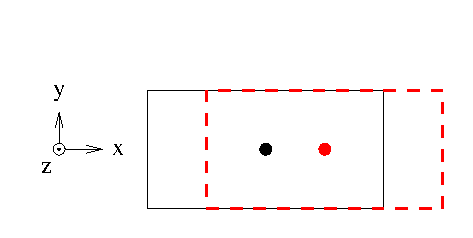
\includegraphics[width=\linewidth]{dof_x.pdf}
  \end{minipage} &
  \begin{minipage}{\linewidth}
    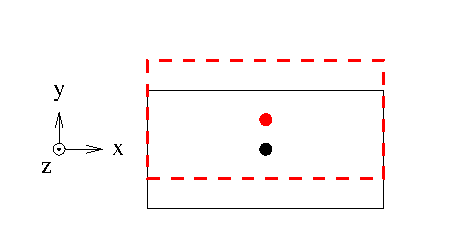
\includegraphics[width=\linewidth]{dof_y.pdf}
  \end{minipage} &
  \begin{minipage}{\linewidth}
    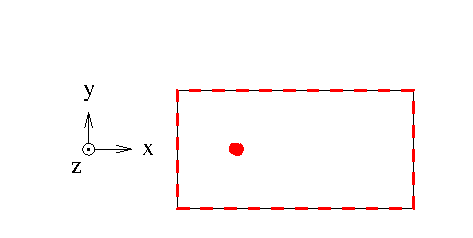
\includegraphics[width=\linewidth]{dof_z.pdf}
  \end{minipage} \\
  \begin{minipage}{\linewidth}
    \begin{center}
      $x$: offset in $r_x$
    \end{center}
  \end{minipage} &
  \begin{minipage}{\linewidth}
    \begin{center}
      $y$: offset in $r_y$
    \end{center}
  \end{minipage} &
  \begin{minipage}{\linewidth}
    \begin{center}
      $z$: sensitive only through angled tracks
    \end{center}
  \end{minipage} \\
  & & \\
  \begin{minipage}{\linewidth}
    \tiny
    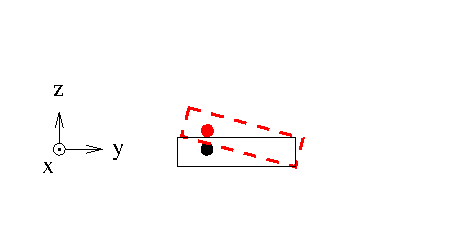
\includegraphics[width=\linewidth]{dof_phix.pdf} \\ \mbox{ }
  \end{minipage} &
  \begin{minipage}{\linewidth}
    \tiny
    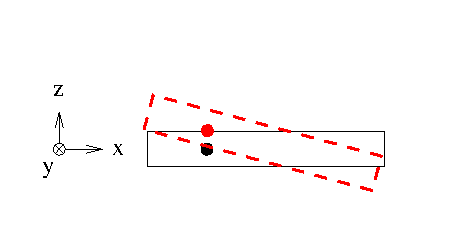
\includegraphics[width=\linewidth]{dof_phiy.pdf} \\ \mbox{ }
  \end{minipage} &
  \begin{minipage}{\linewidth}
    \tiny
    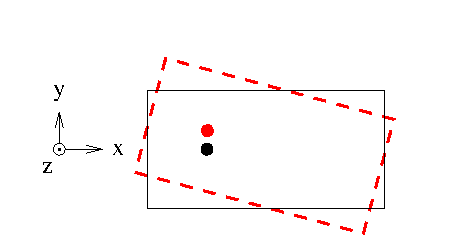
\includegraphics[width=\linewidth]{dof_phiz.pdf} \\ \mbox{ }
  \end{minipage} \\
  \begin{minipage}{\linewidth}
    \begin{center}
      $\phi_x$: $r_y$ linear in $y$ \\ \mbox{ }
    \end{center}
  \end{minipage} &
  \begin{minipage}{\linewidth}
    \begin{center}
      $\phi_y$: $r_x$ linear in $x$ \\ \mbox{ }
    \end{center}
  \end{minipage} &
  \begin{minipage}{\linewidth}
    \begin{center}
      $\phi_z$: $r_x$ linear in $y$ and \\ $r_y$ linear in $x$
    \end{center}
  \end{minipage} \\
  \begin{minipage}{\linewidth}
    \scriptsize
    \begin{center}
      (slope $\propto$ $1 - \cos\phi_x$)
    \end{center}
  \end{minipage} &
  \begin{minipage}{\linewidth}
    \scriptsize
    \begin{center}
      (slope $\propto$ $1 - \cos\phi_y$)
    \end{center}
  \end{minipage} &
  \begin{minipage}{\linewidth}
    \scriptsize
    \begin{center}
      (slope $\propto$ $\sin\phi_z$)
    \end{center}
  \end{minipage}
\end{tabular}
\end{center}
\end{frame}

\begin{frame}
\frametitle{$z$ is important! (slide \only<1>{1}\only<2>{2} of 2)}
Barrel stations 1--3: \only<1>{$z$ is fixed (and misaligned)}\only<2>{$z$ is allowed to float in alignment}
\begin{center}
\only<1>{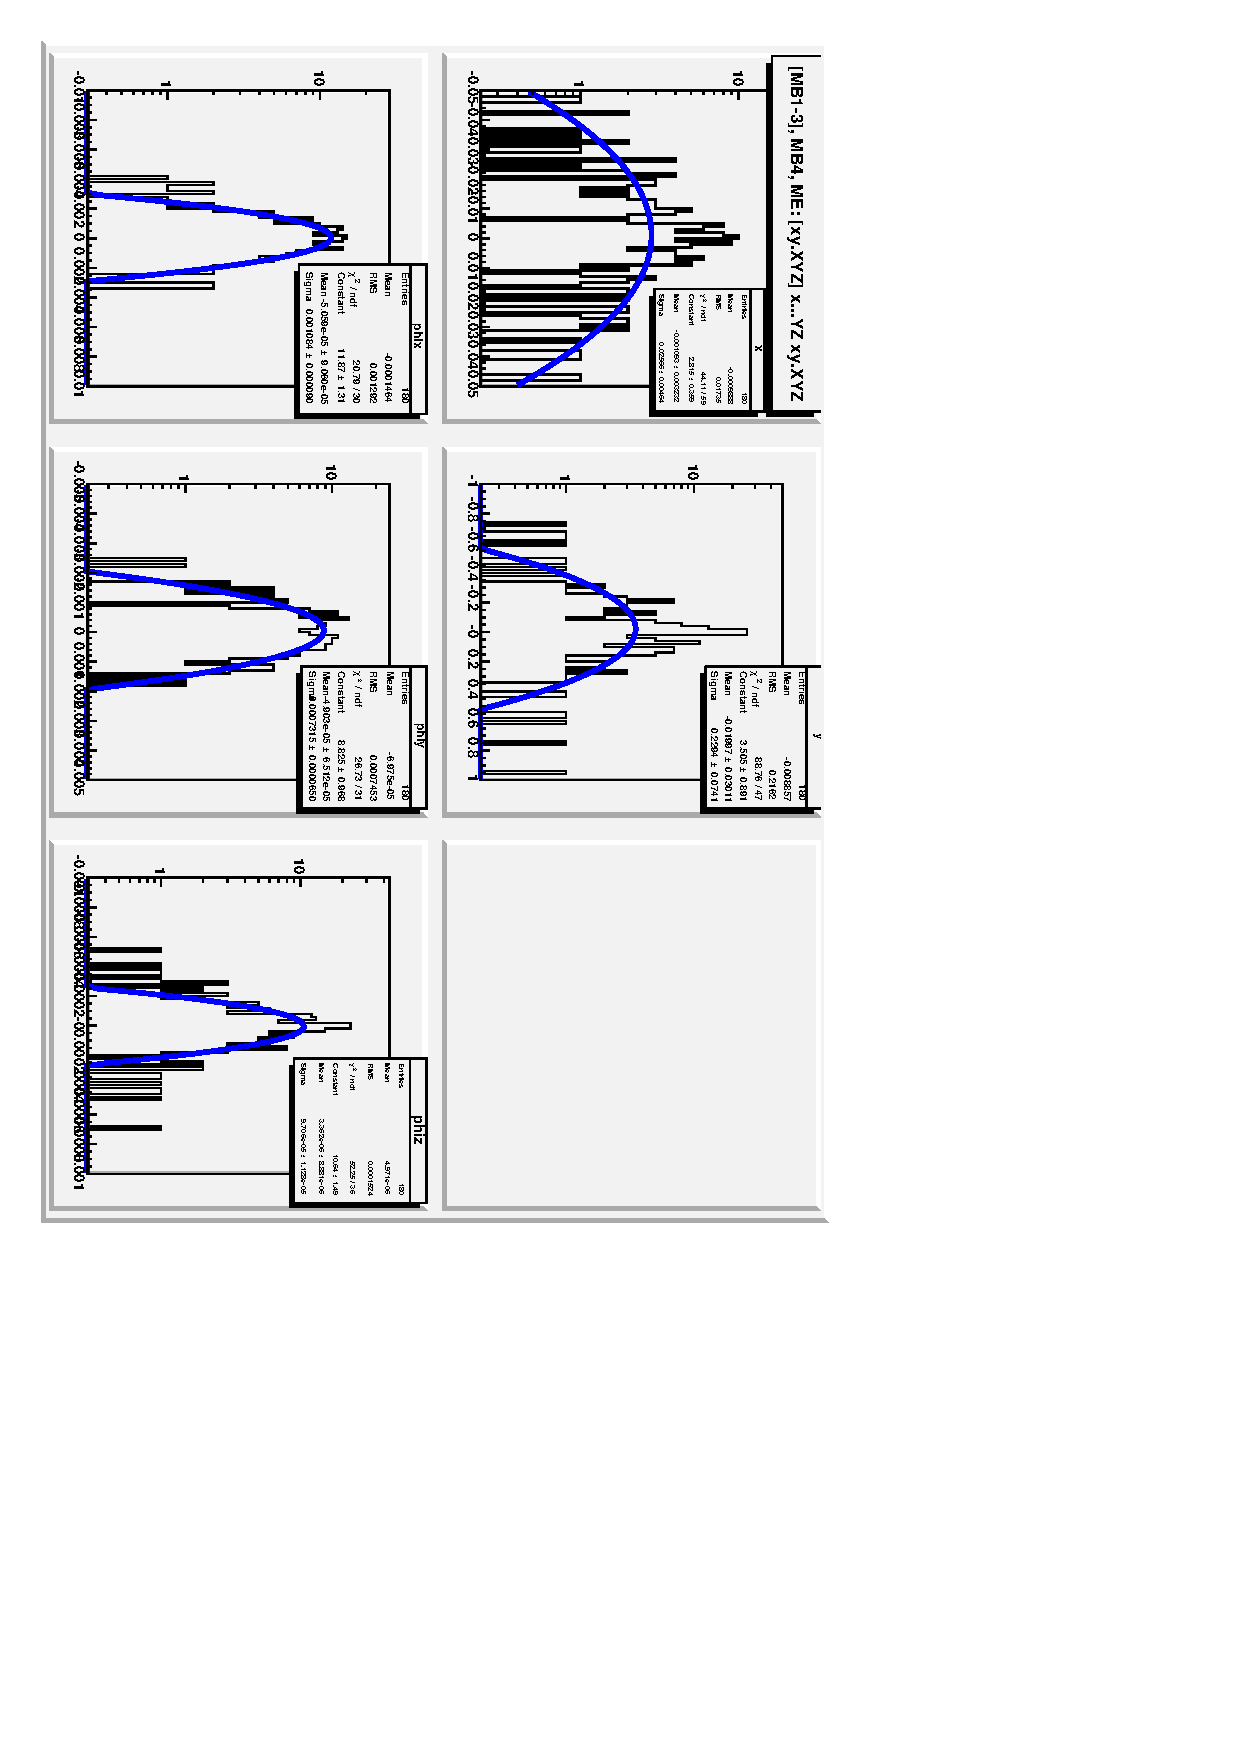
\includegraphics[height=0.8\linewidth, angle=90]{xyXYZ_xYZ_xyXYZ_barrelbulk.pdf}}
\only<2>{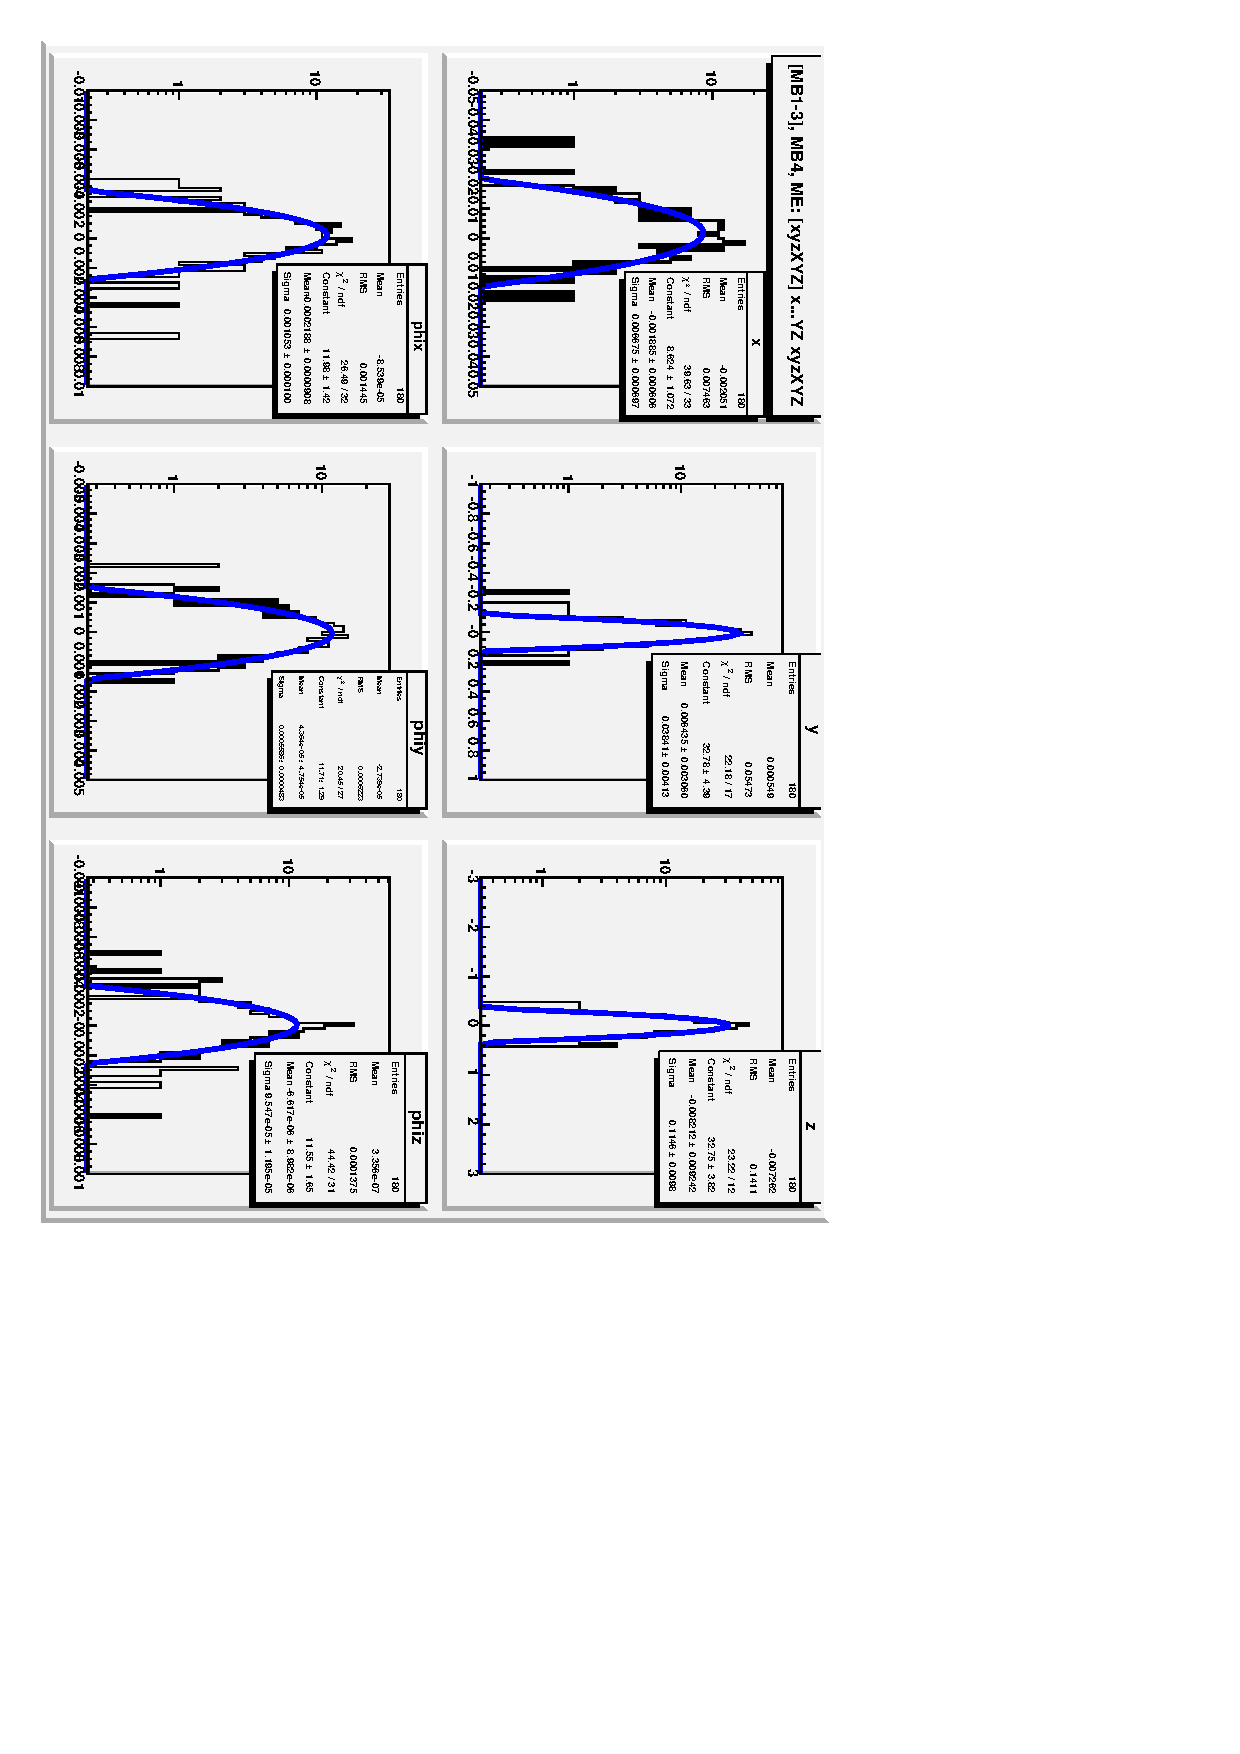
\includegraphics[height=0.8\linewidth, angle=90]{xyzXYZ_xYZ_xyzXYZ_barrelbulk.pdf} \label{pagefive}}

All plots are aligned positions minus correct positions (MC)
\end{center}
\end{frame}

\begin{frame}
\frametitle{Why is that?}
\begin{center}
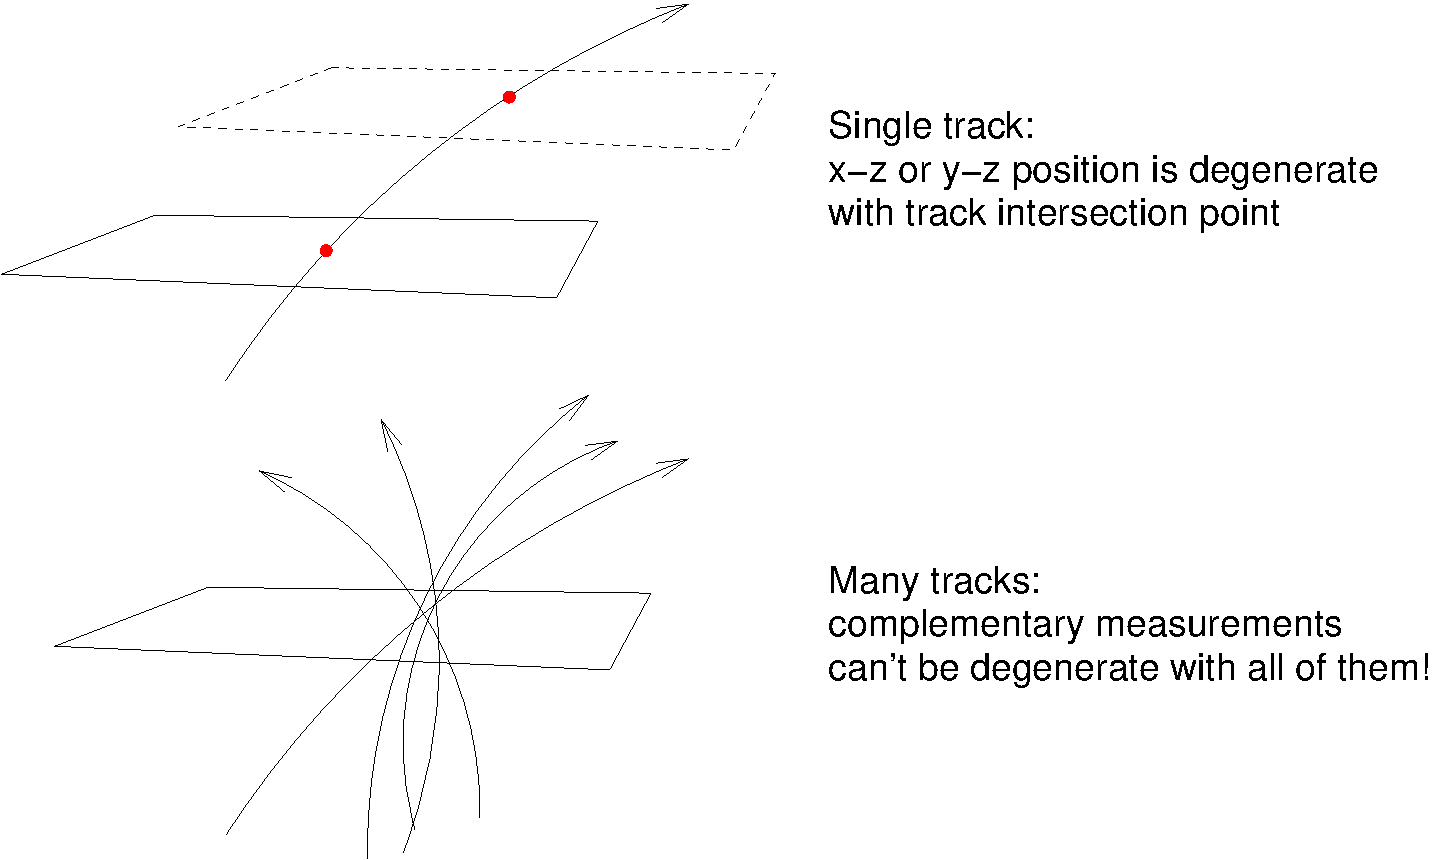
\includegraphics[width=0.85\linewidth]{why_is_that2.pdf}
\end{center}

(Also, chambers are not 2-D surfaces but 6--12 layers thick.  However, the above is a more important part of the explanation.)
\end{frame}

\begin{frame}
\frametitle{Important distinction among barrel chambers}
\begin{itemize}
\item Stations 1--3: full $x$-$y$ measurement (stereo superlayers)
\item Station 4: $x$ only (purely one-dimensional!)
\end{itemize}
\begin{center}
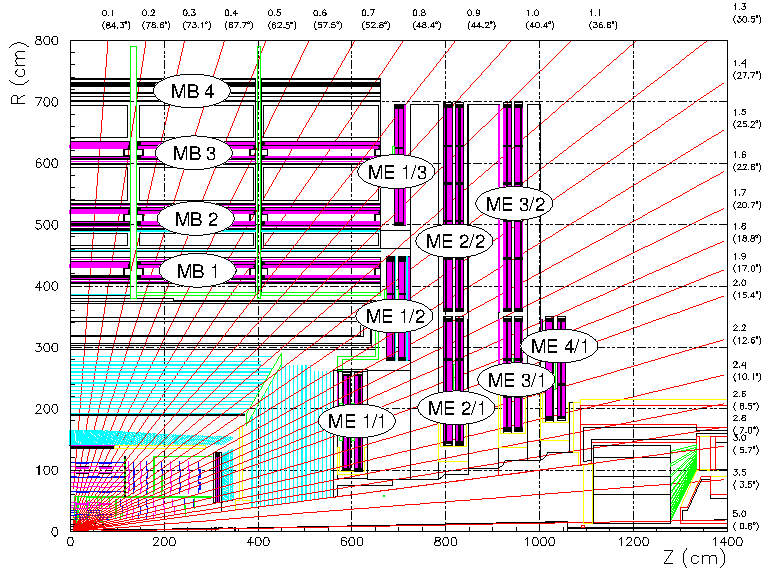
\includegraphics[width=0.75\linewidth]{muon_system_labeled.pdf}
\end{center}
\end{frame}

\begin{frame}
\frametitle{Barrel station 4 (outermost chambers)}
Super-precise $x$ and $\phi_z$ (better intrinsic resolution???) 

$y$, $\phi_x$ are off-limits (cause divergences through numerical error)
\begin{center}
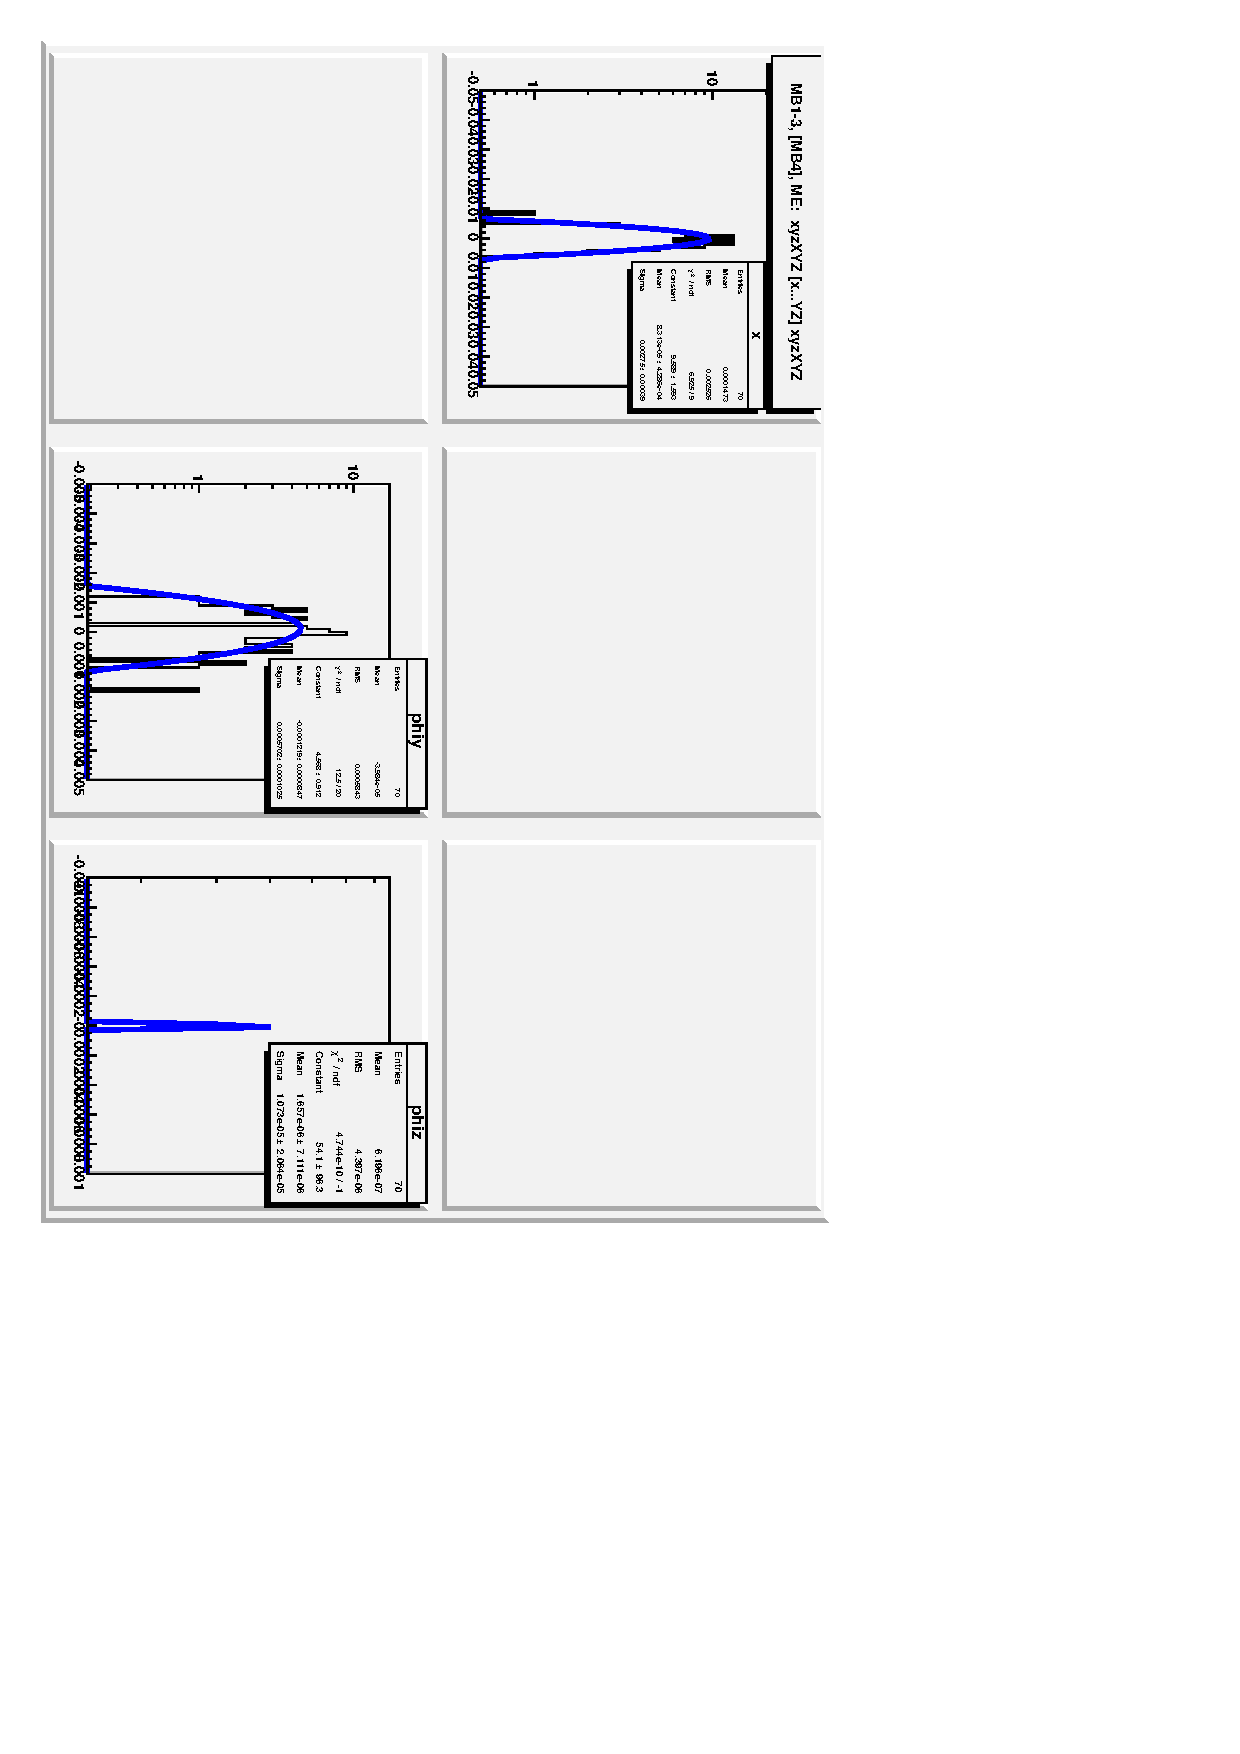
\includegraphics[height=0.75\linewidth, angle=90]{xyzXYZ_xYZ_xyzXYZ_barrelsurface.pdf}
\end{center}
what about $z$?  hmmm\ldots I didn't try that\ldots
\end{frame}

\begin{frame}
\frametitle{Barrel alignment results}
\hspace{1.5 cm} Stations 1--3
\begin{center}
\begin{tabular}{c c | c c}
\hline\hline
$x$ & 67 $\mu$m & 1.05 mrad & $\phi_x$ \\
$y$ & 384 $\mu$m & 0.56 mrad & $\phi_y$ \\
$z$ & 1.15 mm & 0.095 mrad & $\phi_z$ \\
\hline\hline
\end{tabular}
\end{center}
\mbox{ } \hfill \ldots and very Gaussian!!!  Few outliers (see p.\ \pageref{pagefive})!

\vfill
\hspace{1.5 cm} Station 4
\begin{center}
\begin{tabular}{c c | c c}
\hline\hline
$x$ & 28 $\mu$m &  \\
    &           & 0.57 mrad & $\phi_y$ \\
    &           & 0.004 mrad & $\phi_z$ \\
\hline\hline
\end{tabular}

\vspace{0.2 cm}
If $\phi_y$ is fixed, $x$ $\to$ 12 $\mu$m

(unnecessary ultraprecision)
\end{center}
\end{frame}

\begin{frame}
\frametitle{Full evolution of endcap: $x$....$\phi_z$ (1/5)}
\begin{center}
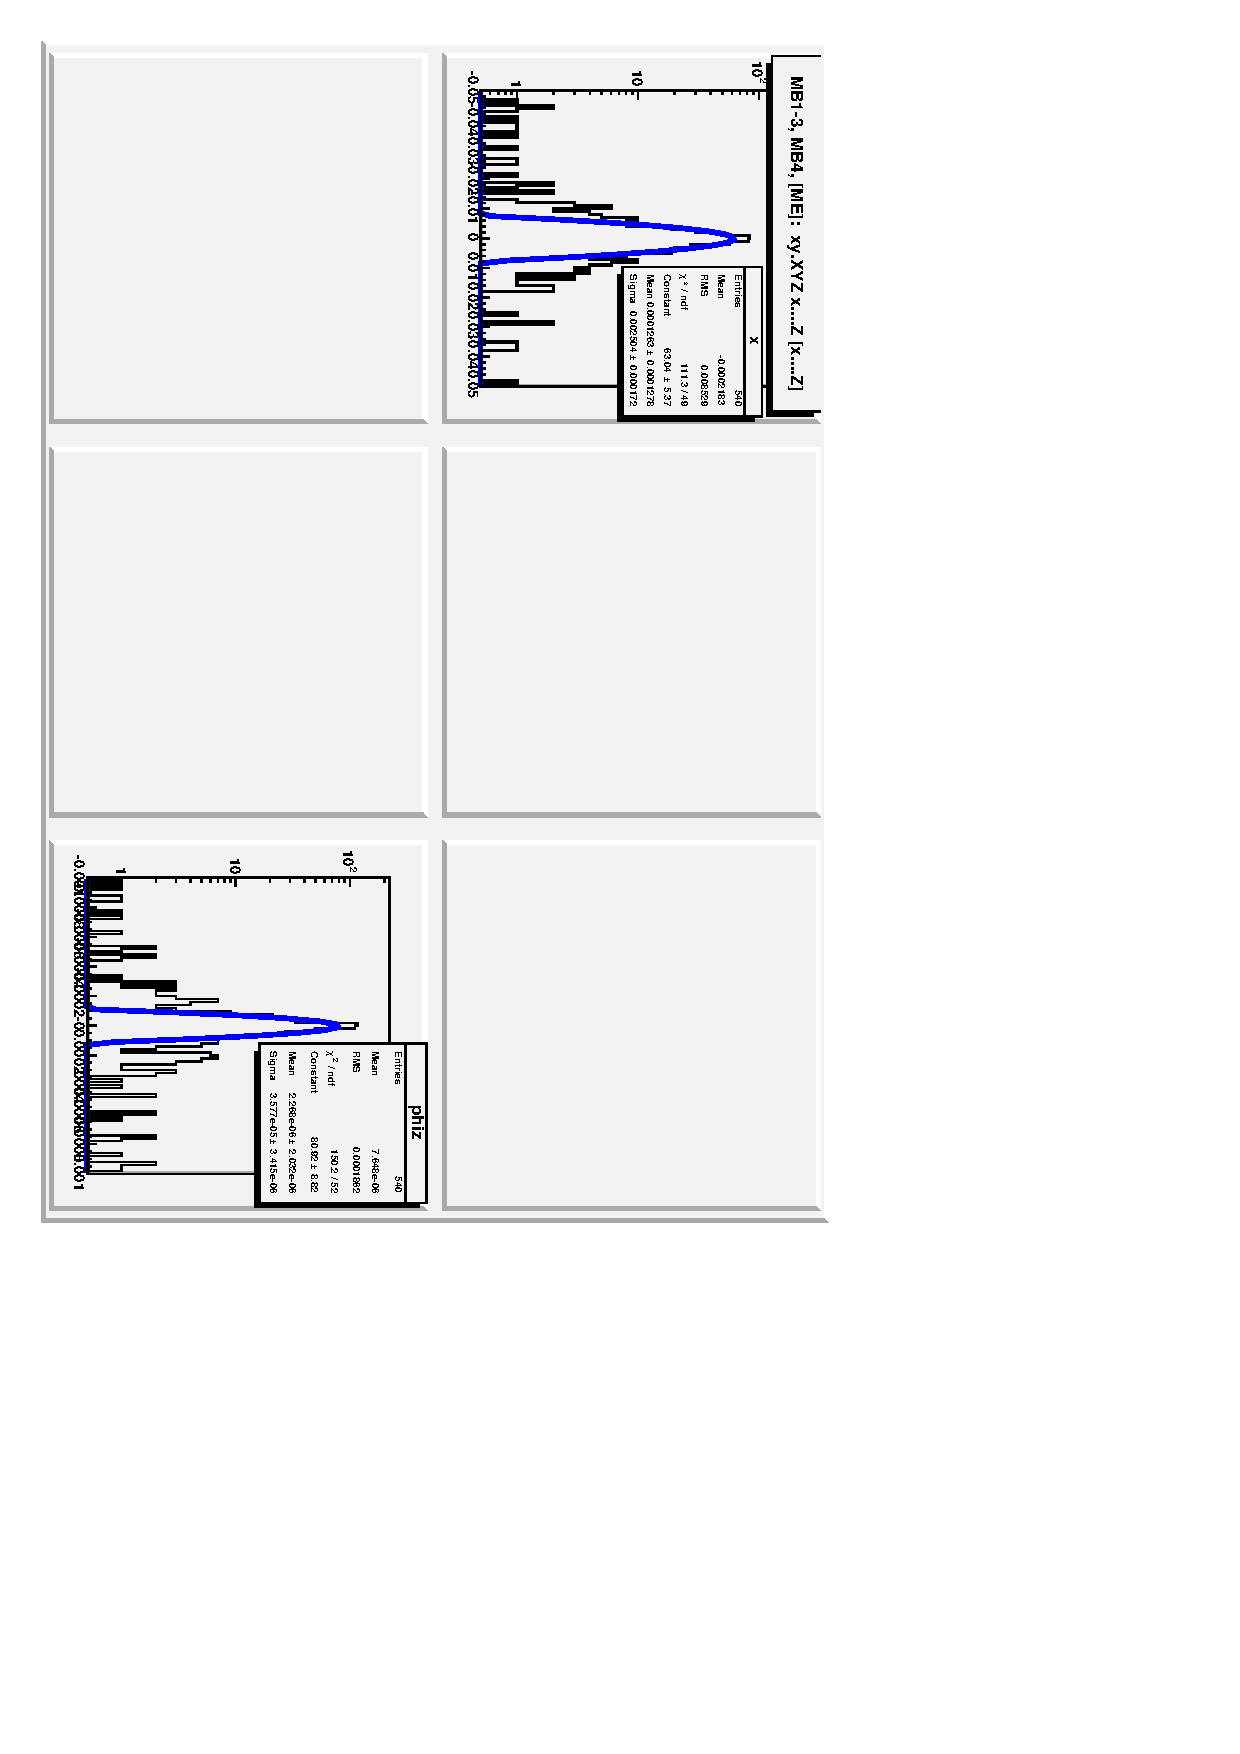
\includegraphics[height=\linewidth, angle=90]{xyXYZ_xZ_xZ_endcap.pdf}
\end{center}
\end{frame}

\begin{frame}
\frametitle{Full evolution of endcap: $xy$...$\phi_z$ (2/5)}
\begin{center}
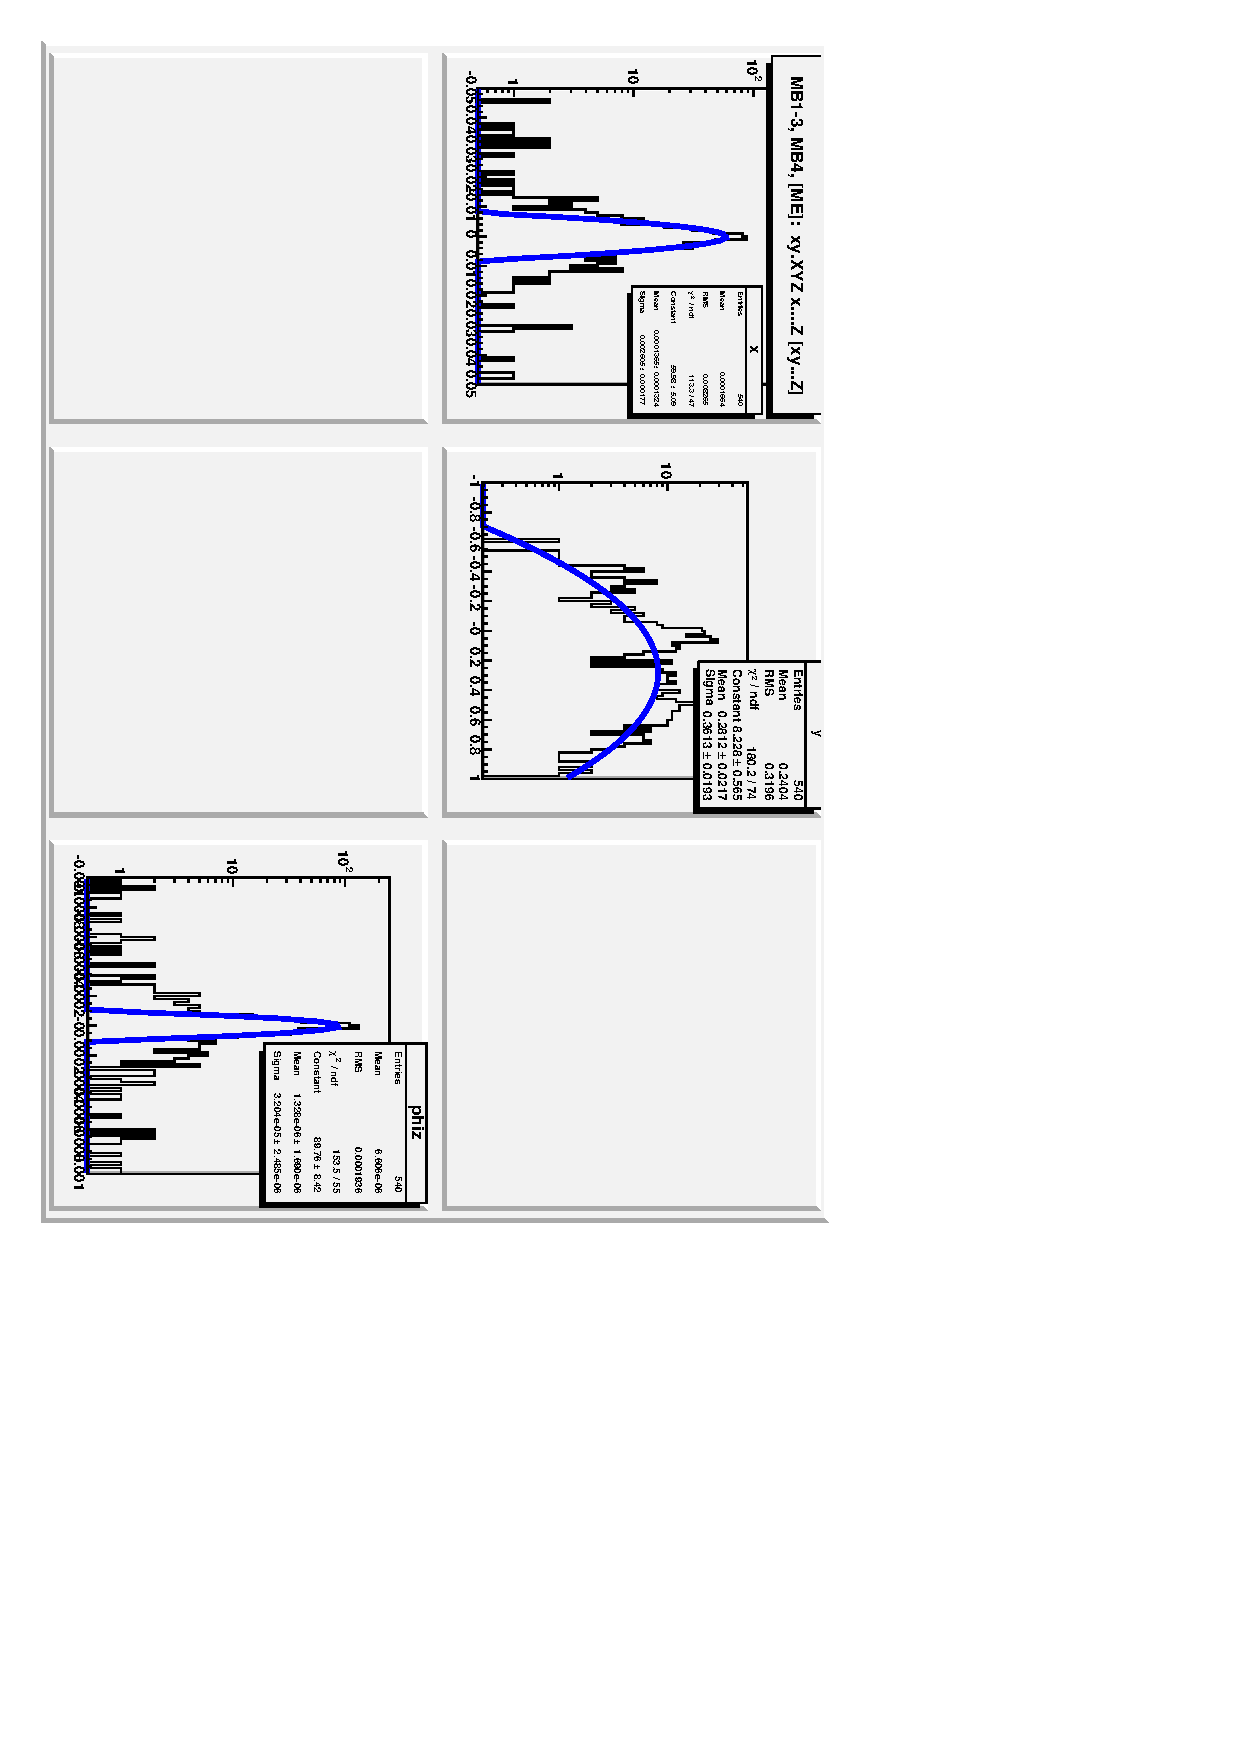
\includegraphics[height=\linewidth, angle=90]{xyXYZ_xZ_xyZ_endcap.pdf}
\end{center}
\end{frame}

\begin{frame}
\frametitle{Full evolution of endcap: $xy$..$\phi_y\phi_z$ (3/5)}
\begin{center}
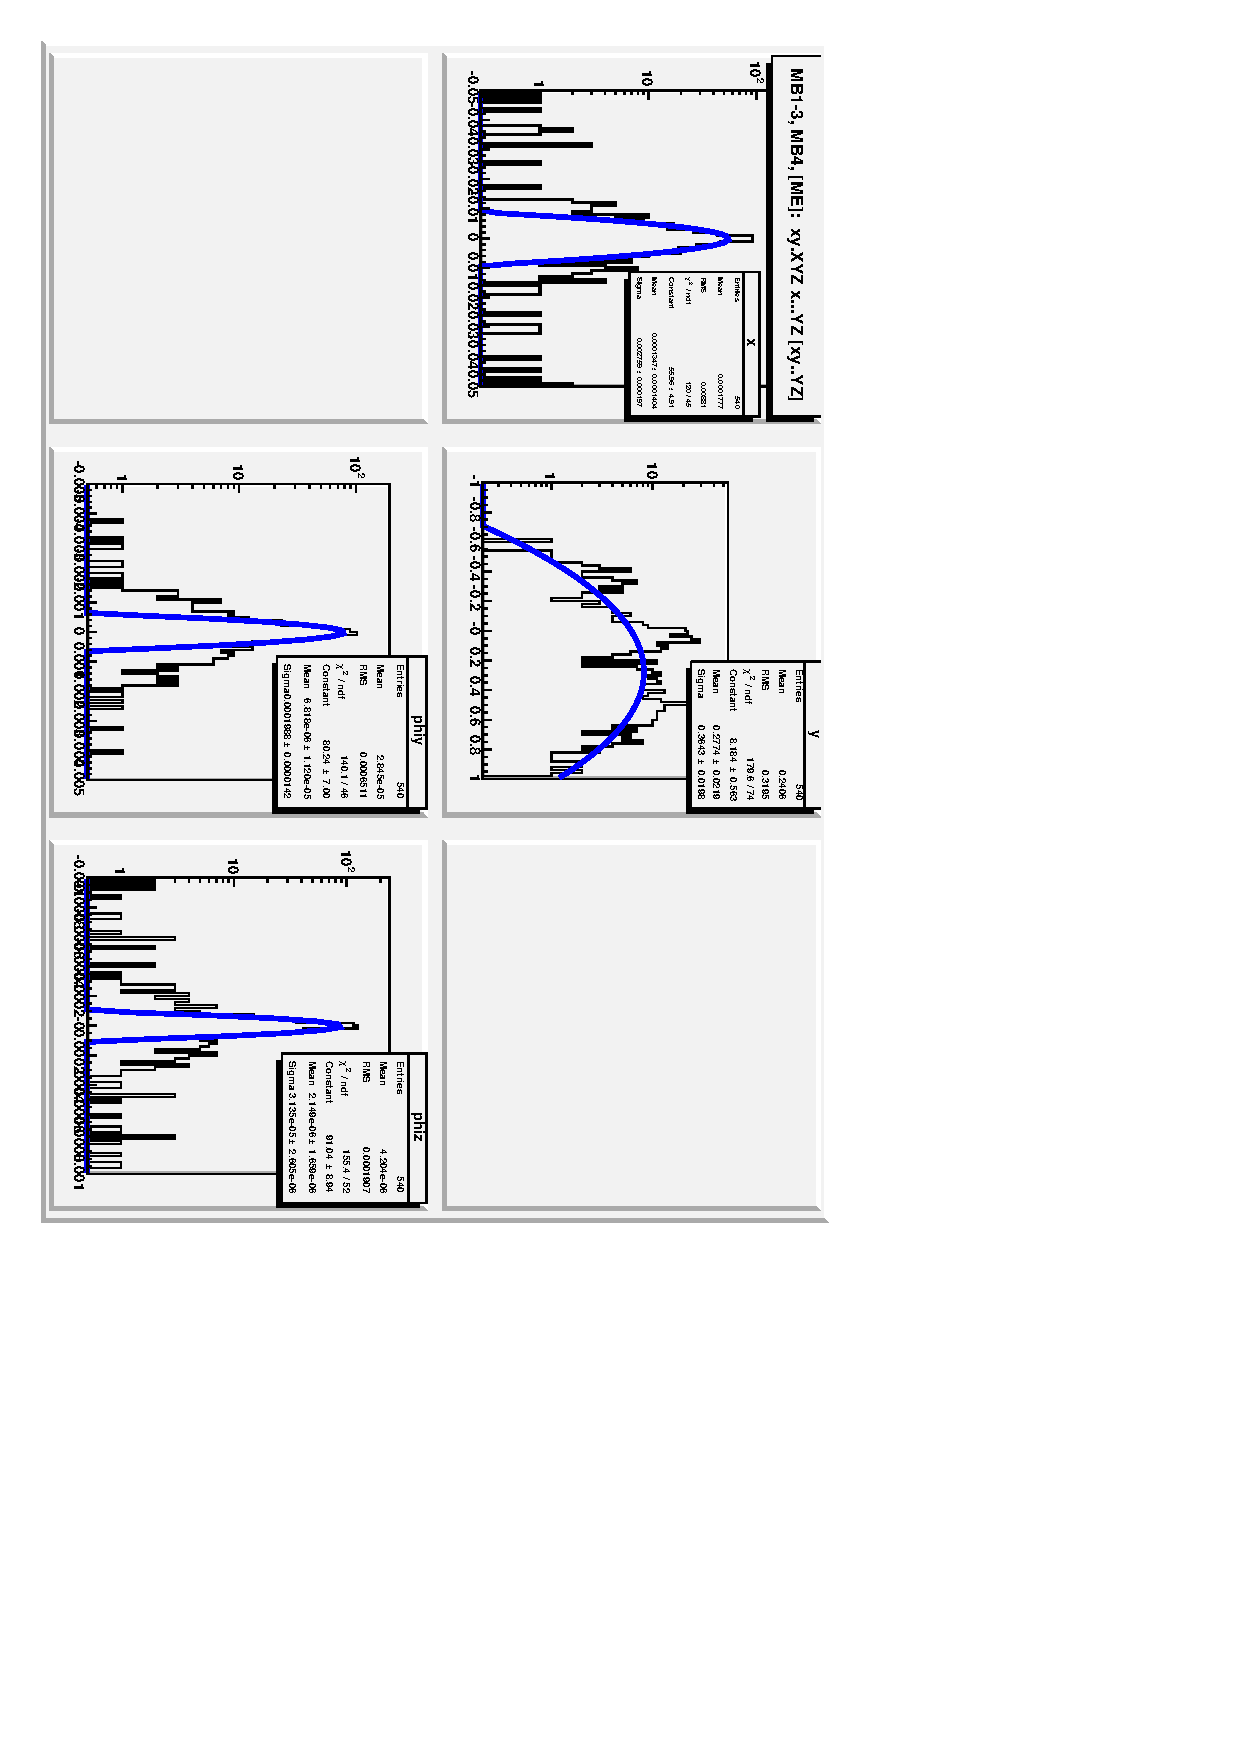
\includegraphics[height=\linewidth, angle=90]{xyXYZ_xYZ_xyYZ_endcap.pdf}
\end{center}
\end{frame}

\begin{frame}
\frametitle{Full evolution of endcap: $xy$.$\phi_x\phi_y\phi_z$ (4/5)}
\begin{center}
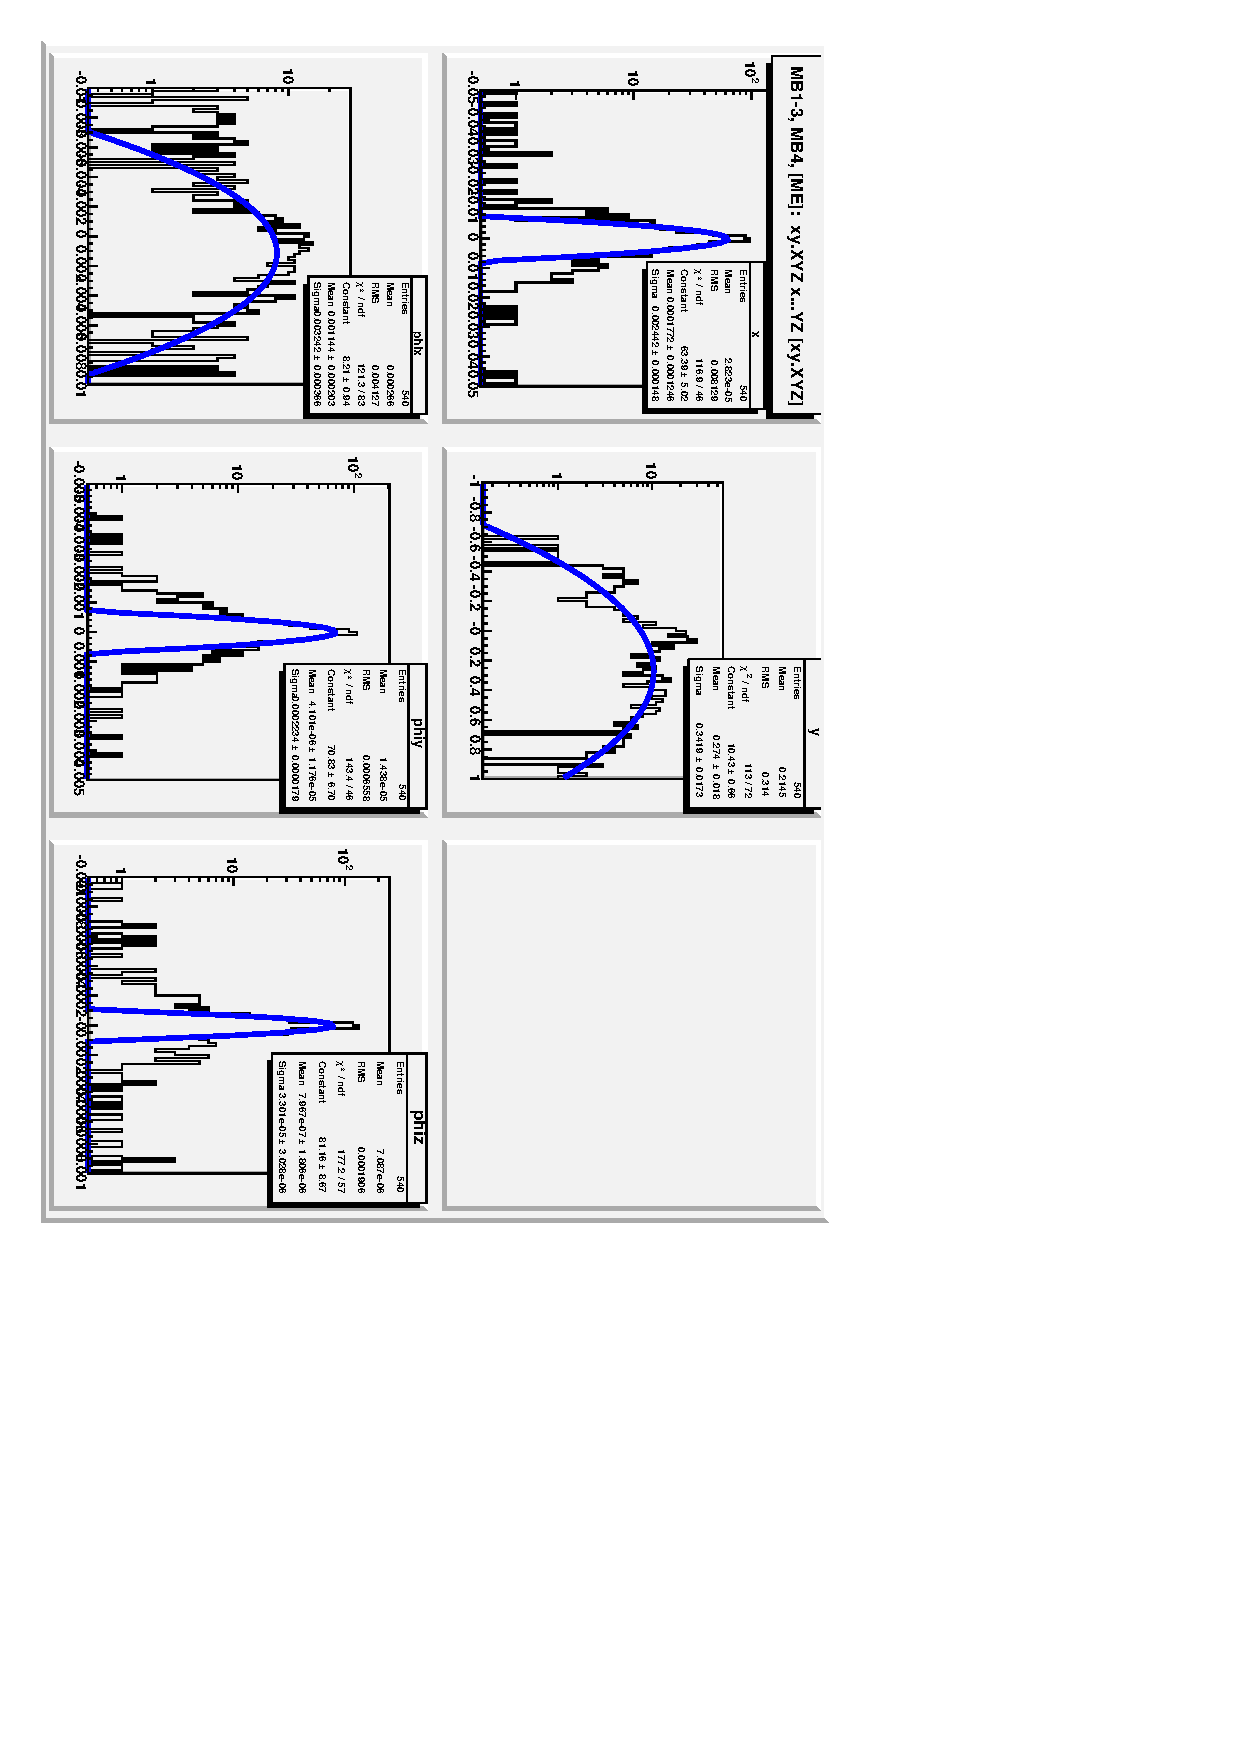
\includegraphics[height=\linewidth, angle=90]{xyXYZ_xYZ_xyXYZ_endcap.pdf}
\end{center}
\end{frame}

\begin{frame}
\frametitle{Full evolution of endcap: $xyz\phi_x\phi_y\phi_z$ (5/5)}
\begin{center}
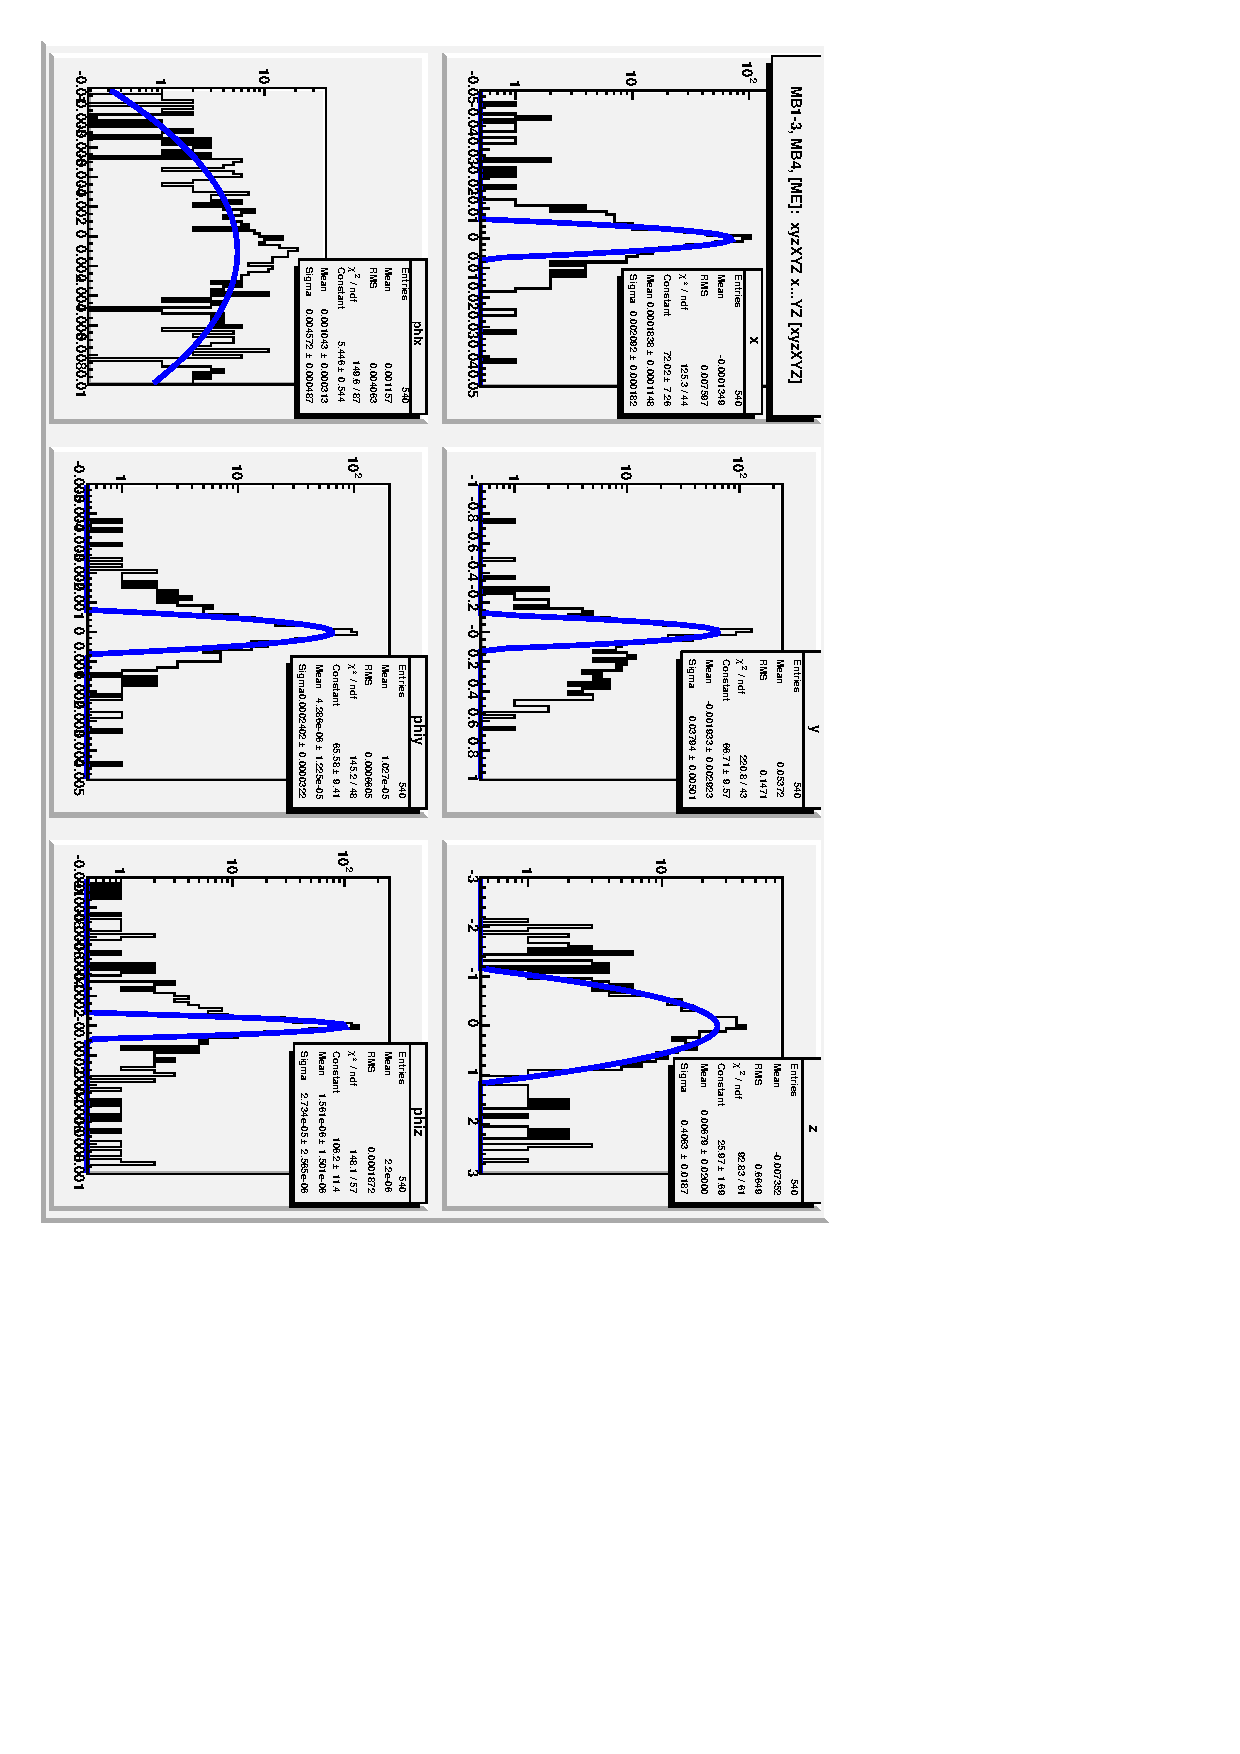
\includegraphics[height=\linewidth, angle=90]{xyzXYZ_xYZ_xyzXYZ_endcap.pdf}
\end{center}
\end{frame}

\begin{frame}
\frametitle{Wow!  What's going on?}
\vspace{-0.5 cm}
\begin{columns}
\column{0.6\linewidth}

Allowing $z$ to float helps $y$ enormously, though there's a strange asymmetric secondary distribution.

\column{0.35\linewidth}
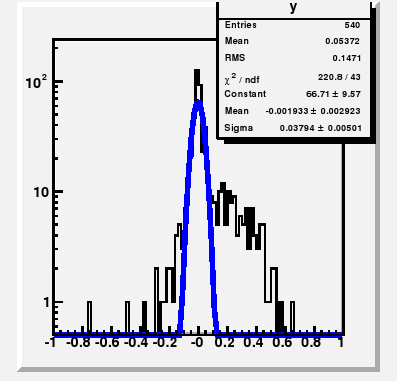
\includegraphics[width=\linewidth]{just_endcap_y.png}
\end{columns}

\vfill
\begin{columns}
\column{0.6\linewidth}

I asked our spiffy analysis tool which chambers have $y_{\mbox{\scriptsize misalign}}$ $>$ 2~mm

\vspace{0.5 cm}
They're (almost) all in ME1/1!

\column{0.3\linewidth}
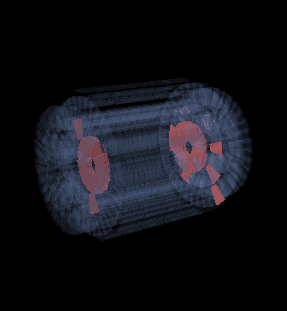
\includegraphics[width=\linewidth]{wierd_bump_locations2.png}
\end{columns}
\end{frame}

\begin{frame}
\frametitle{Is ME1/1 one-dimensional?  NO.  (I didn't think so.)}
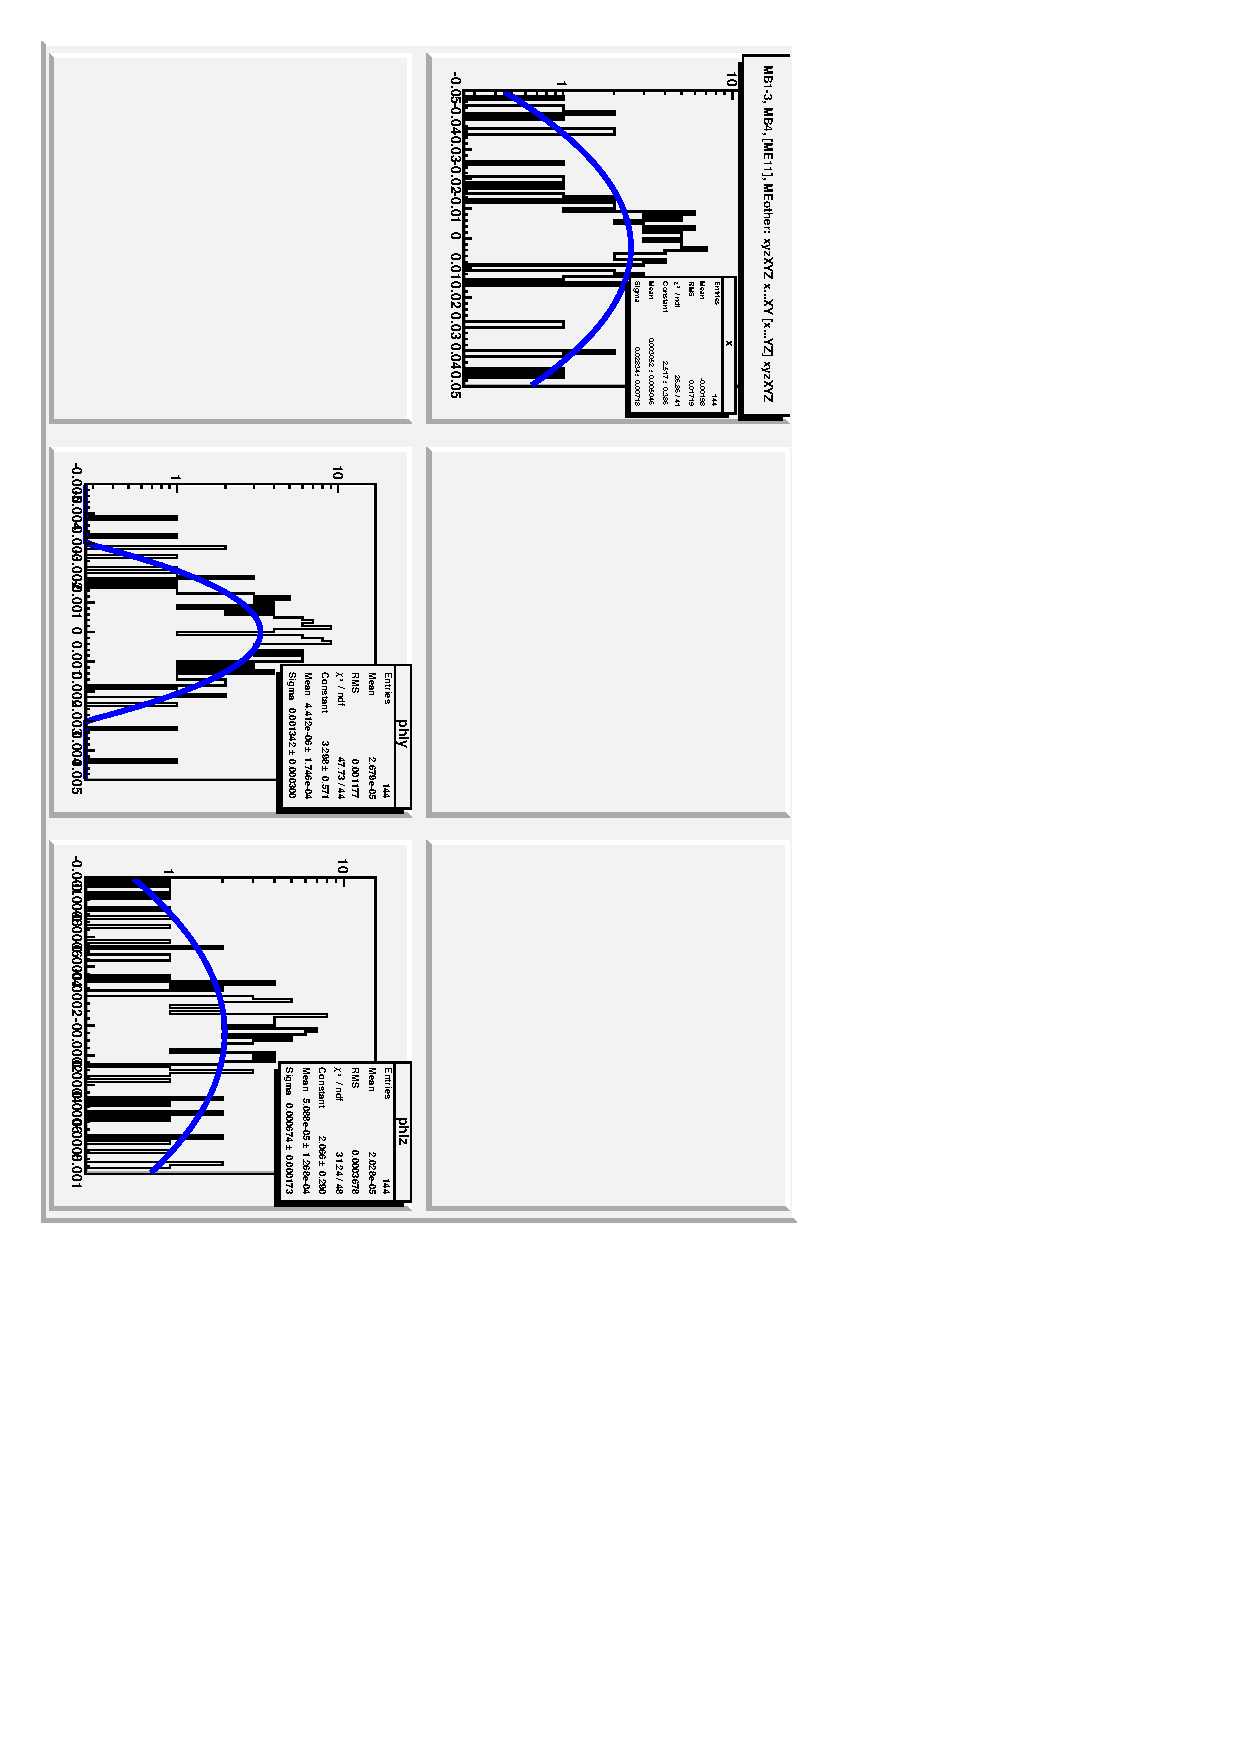
\includegraphics[height=\linewidth, angle=90]{optimized_tight_endcapme11.pdf}
\end{frame}

\begin{frame}
\frametitle{The $y$ residual distributions are a {\it little} asymmetric\ldots}
\begin{center}
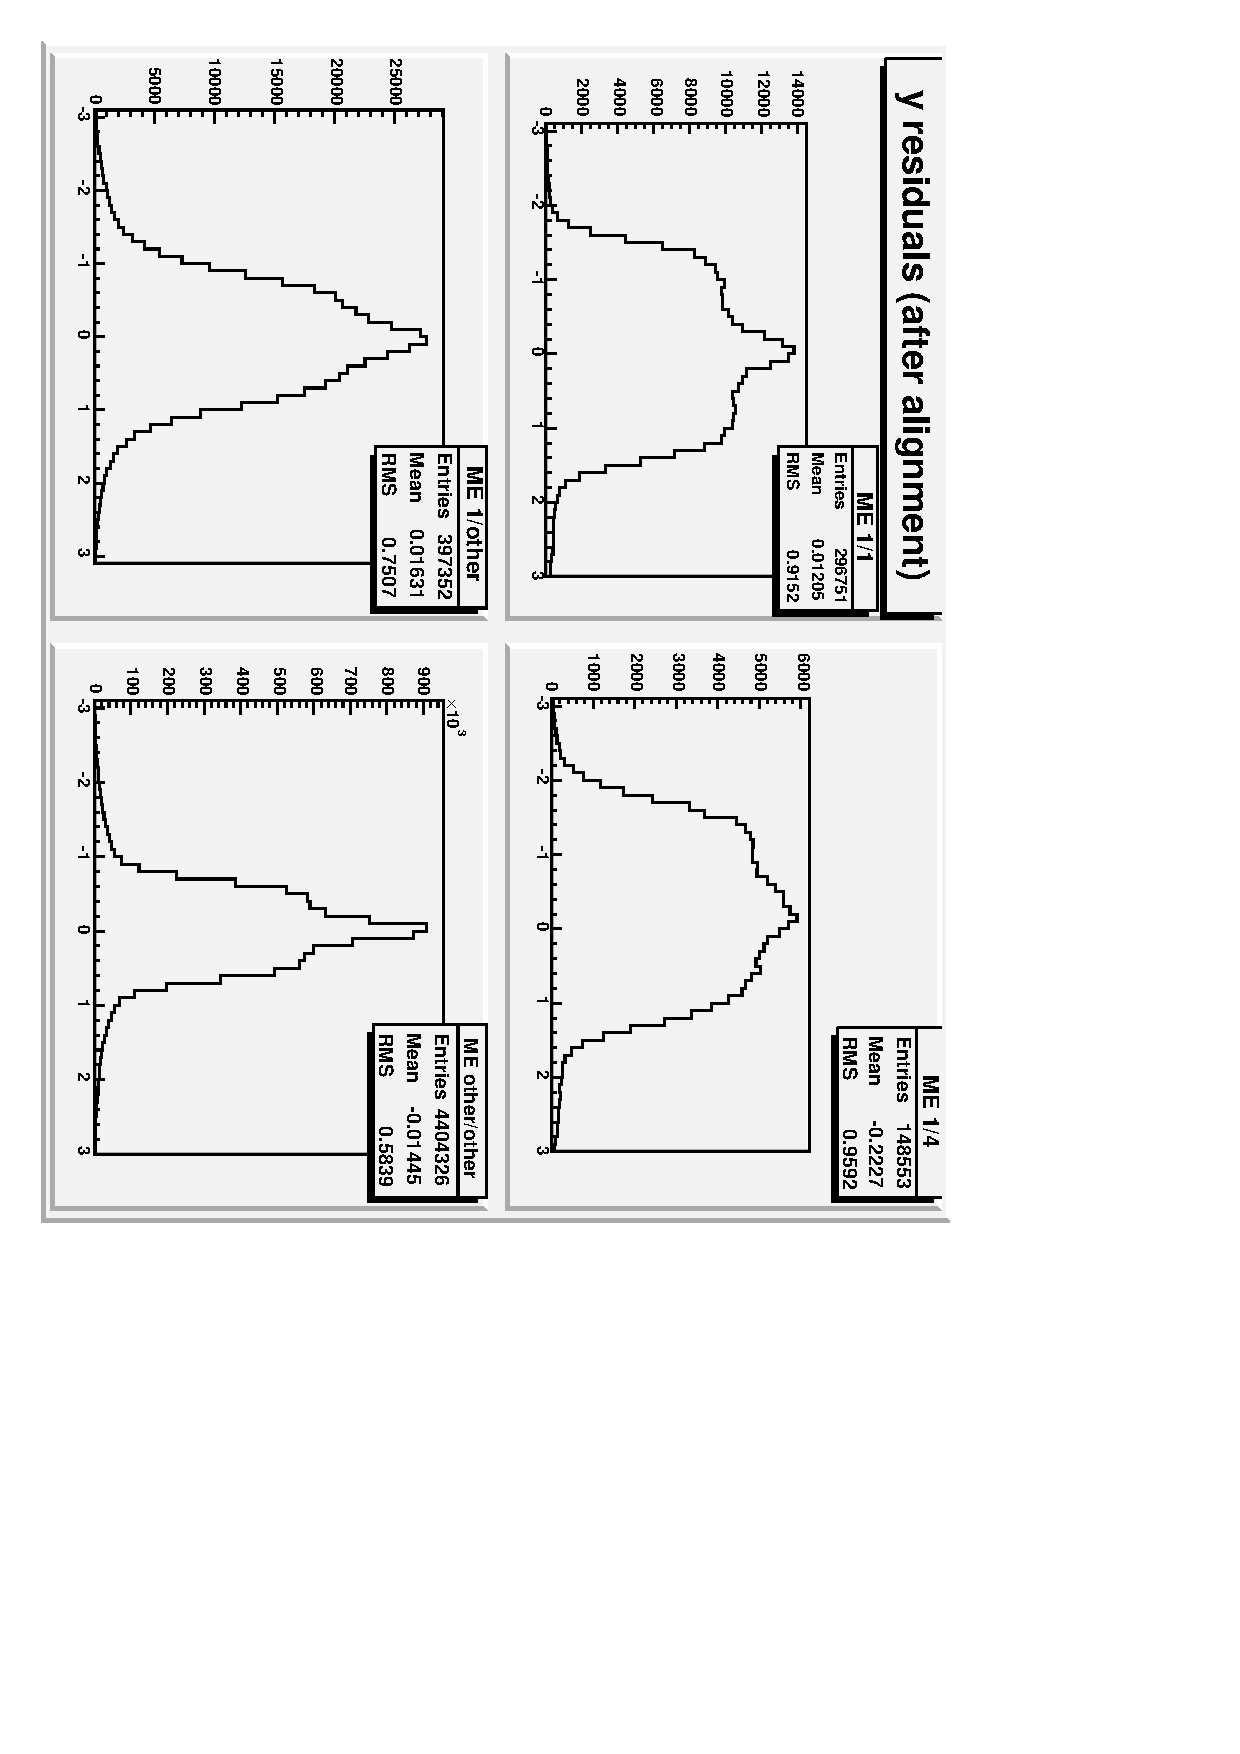
\includegraphics[height=0.85\linewidth, angle=90]{y_residuals.pdf}
\end{center}
\end{frame}

\begin{frame}
\frametitle{The $x$ residual distributions, for completeness}
\begin{center}
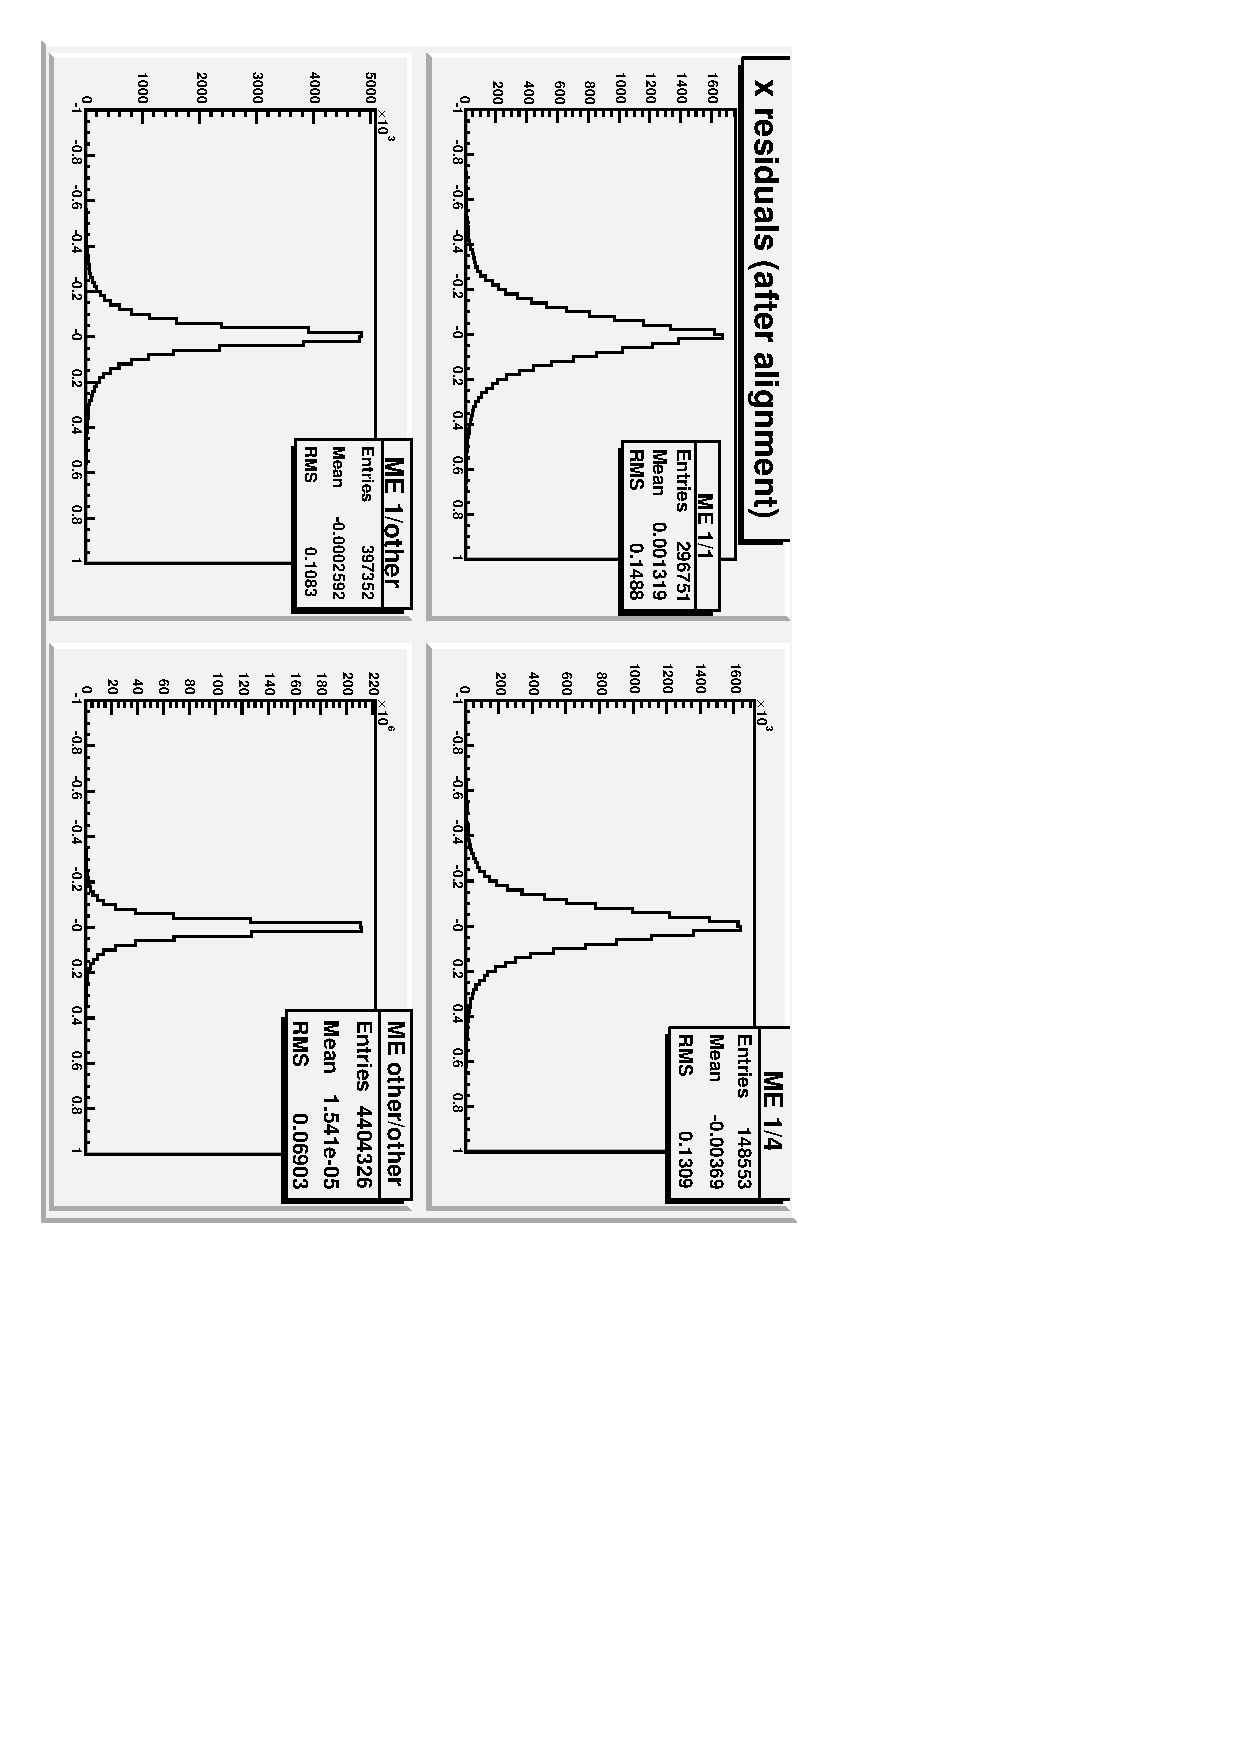
\includegraphics[height=\linewidth, angle=90]{x_residuals.pdf}
\end{center}
\end{frame}

\begin{frame}
\frametitle{Endcap without ME1/1: $xyz$.$\phi_y\phi_z$}
\begin{center}
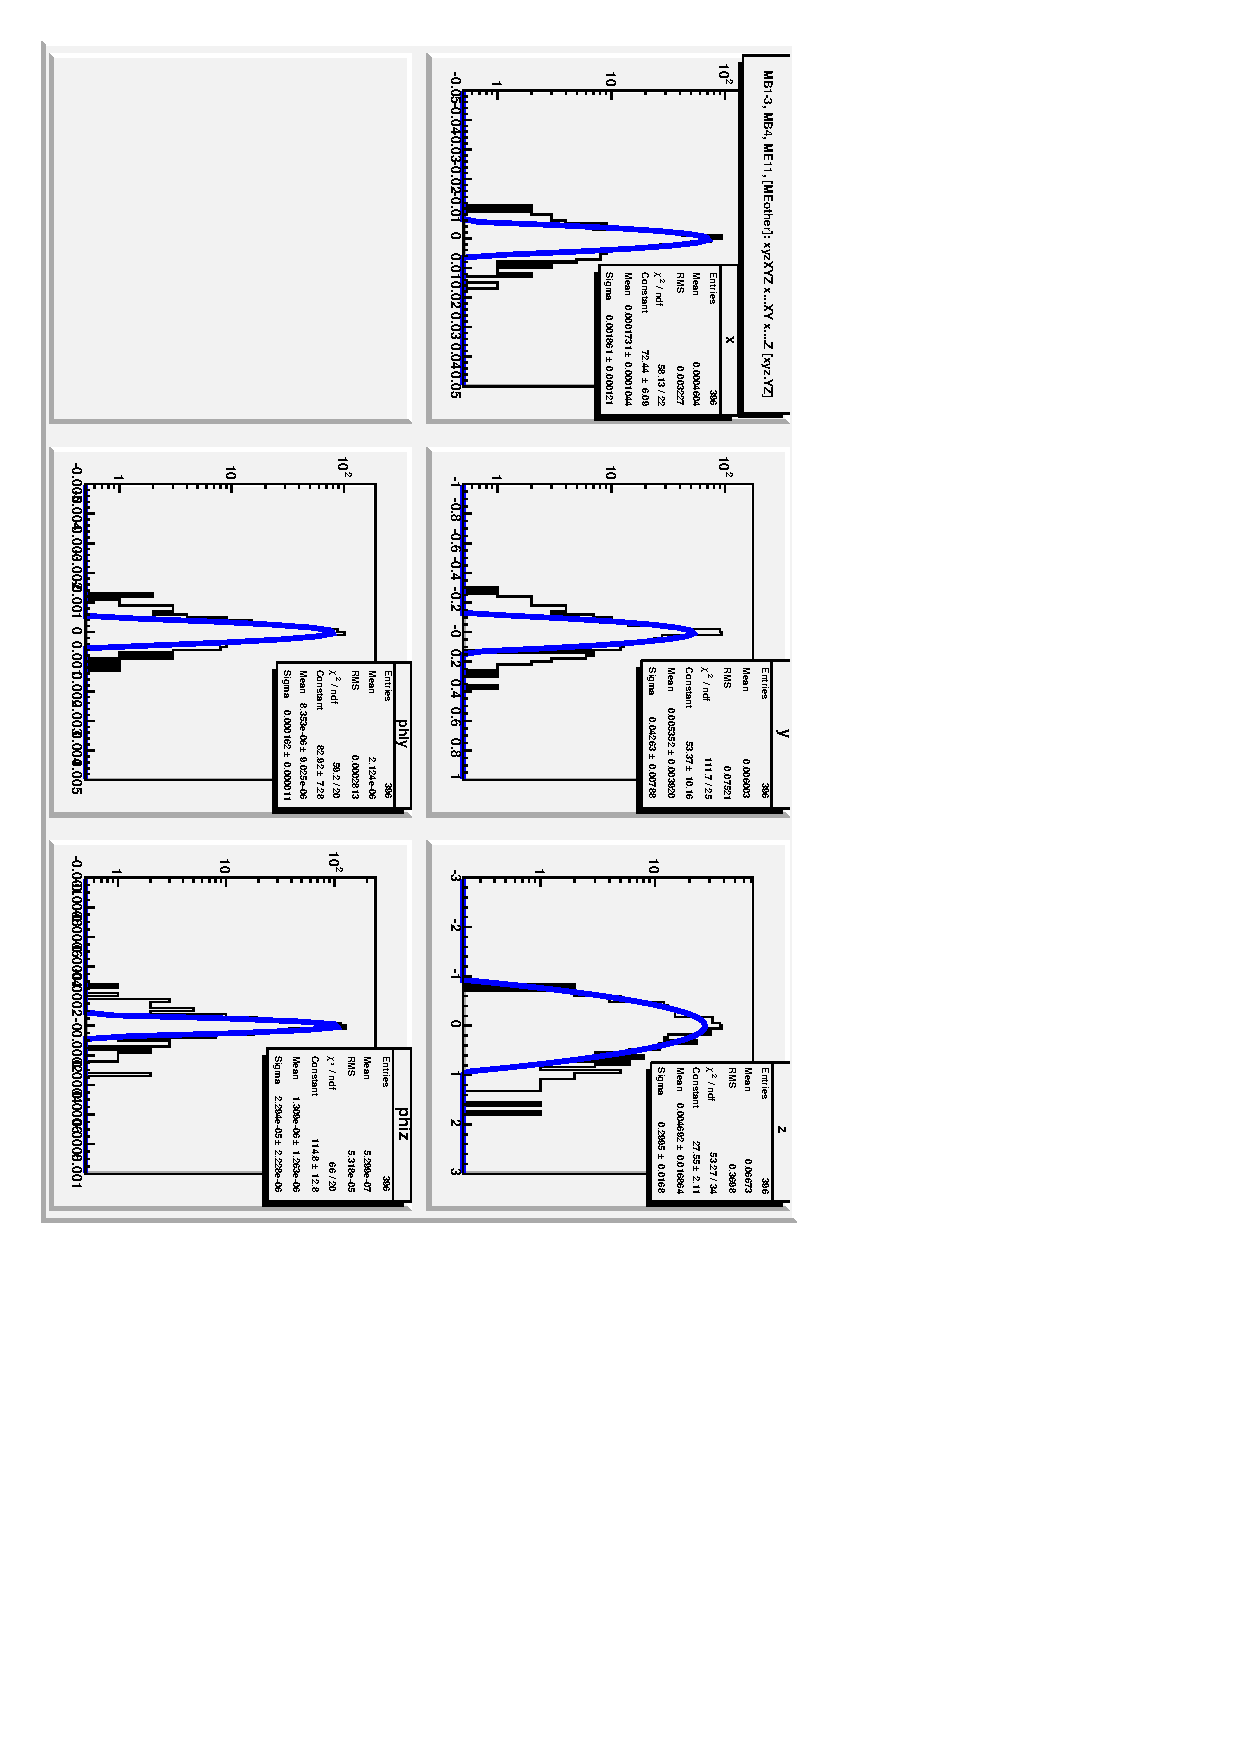
\includegraphics[height=\linewidth, angle=90]{optimized_loose_endcapother.pdf}
\end{center}
\end{frame}

\begin{frame}
\frametitle{Endcap without ME1/1: $xyz\phi_x\phi_y\phi_z$}
\begin{center}
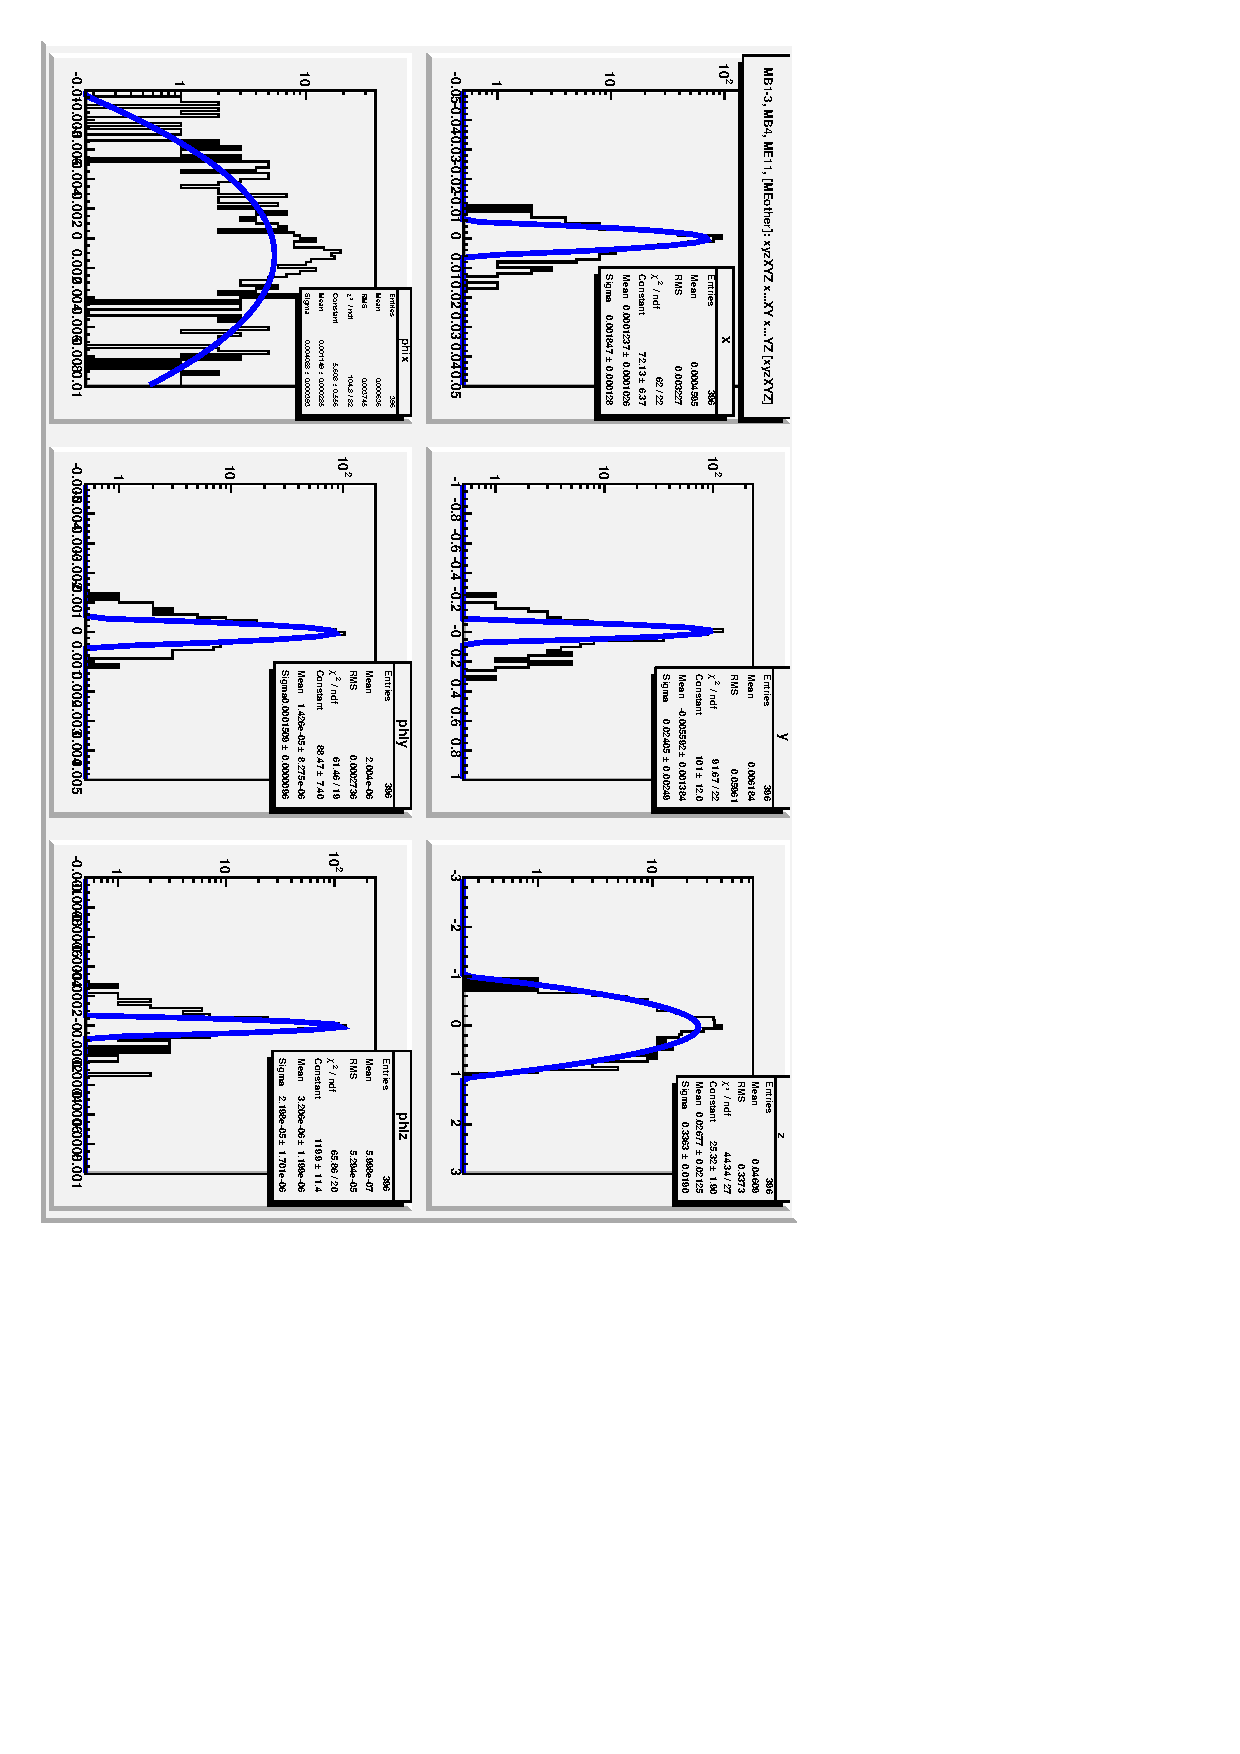
\includegraphics[height=\linewidth, angle=90]{optimized_tight_endcapother.pdf}
\end{center}
\end{frame}

\begin{frame}
\frametitle{Endcap without ME1/1 results}

Resolution is nearly Gaussian--- the long tails are gone
\begin{center}
\begin{tabular}{c | c c}
\hline\hline
\mbox{\hspace{1 cm}} & fitted core & standard deviation \\\hline
$x$ & 19 $\mu$m & 32 $\mu$m \\
$y$ & 240 $\mu$m & 596 $\mu$m \\
$z$ & 3.0 mm & 3.7 mm \\\hline
$\phi_x$ & {\it 4.1 mrad} & {\it 3.7 mrad} \\
$\phi_y$ & 0.16 mrad & 0.28 mrad \\
$\phi_z$ & 0.03 mrad & 0.05 mrad \\
\hline\hline
\end{tabular}
\end{center}

\vfill After alignment $\phi_x$ is worse than before.
However, excluding $\phi_x$ from the fit broadens $y$ resolution to
240~$\mu$m~core, 596~$\mu$m~stdev.  Tie breaker: momentum resolution.  Coming soon.

\vfill
{\bf And} these include internal layer-by-layer misalignments (100's of $\mu$m, as measured by Karoly)!
\end{frame}

\begin{frame}
\frametitle{Summary, conclusions, and questions}
\begin{itemize}
\item<1-> With high-statistics, no miscalibration, no tracker misalignment: we
see beautiful resolution in all but ME1/1

\item<1-> Presumably we can get ME1/1 right by applying some physical
insight (worked for MB4), but I think I'm lacking knowledge of the
system

\item<2-> For instance, ``ME1/1'' and ``ME1/4'' (in software) describe two
parts of some kind of ``double-chamber'' system.  How does that work exactly?

\item<2-> Alignment software allows ``ME1/1'' and ``ME1/4'' to
float independently, which is probably wrong.  Is it disastrously
wrong?

\item<3-> ME1/1 $y$ distribution has the same asymmetry as the rest of the
endcap did when $z$ was misaligned and not allowed to float\ldots

\end{itemize}
\label{numpages}
\end{frame}

\end{document}
